% Modelo de TCC do Bacharelado em Ciência da Computação da UNIFESP 
% Baseado no Modelo de Documentos Academicos do ABNTex2  

  \documentclass[	12pt, Times, openright, twoside, a4paper, english, brazil]{abntex2}

% ---
% Pacotes fundamentais 
% ---
  \usepackage{cmap}				% Mapear caracteres especiais no PDF
  %\usepackage{lmodern}			% Usa a fonte Latin Modern			
  \usepackage{times}
  \usepackage[T1]{fontenc}			% Selecao de codigos de fonte.
  \usepackage[utf8]{inputenc}		% Codificacao do documento (conversão automática dos acentos)
  \usepackage{lastpage}			% Usado pela Ficha catalográfica
  %\usepackage{natbib}
  \usepackage{indentfirst}			% Indenta o primeiro parágrafo de cada seção.
  \usepackage{color}				% Controle das cores
  \usepackage{graphicx}			% Inclusão de gráficos
  % ---
  \usepackage[portuguese, ruled, linesnumbered]{algorithm2e} %Peseudocodigo
  \usepackage{amssymb} %checkmarker
% ---
% Pacotes de citações
% ---
  \usepackage[brazilian,hyperpageref]{backref}	 % Paginas com as citações na bibl
  \usepackage[alf]{abntex2cite}	% Citações padrão ABNT

% --- 
% CONFIGURAÇÕES DE PACOTES
% --- 

% ---
% Configurações do pacote backref
% Usado sem a opção hyperpageref de backref
  \renewcommand{\backrefpagesname}{Citado na(s) página(s):~}
  % Texto padrão antes do número das páginas
  \renewcommand{\backref}{}
  % Define os textos da citação
  \renewcommand*{\backrefalt}[4]{
  	\ifcase #1 %
  		Nenhuma citação no texto.%
  	\or
  		Citado na página #2.%
  	\else
  		Citado #1 vezes nas páginas #2.%
  	\fi}%
  % ---

  % numeração de figuras e elas 
  \counterwithout{figure}{section}
  \counterwithout{table}{section}

  %\renewcommand\tablename{Tabela{\arabic{chapter}.}}


% ---
% Informações de dados para CAPA e FOLHA DE ROSTO
% ---
  \titulo{ANÁLISE DE DEMANDA VIA INTELIGÊNCIA ARTIFICIAL NO RESTAURANTE UNIVERSITÁRIO DO INSTITUTO CENTRAL DE TECNOLOGIA DA UNIFESP}
  \autor{Douglas Diniz Landim}
  \local{São José dos Campos, SP}
  \data{Março de 2018}
  \orientador{Prof. Dr. Vinicius Veloso}
  %\coorientador{Prof. Dr. }
  \instituicao{%
    Universidade Federal de São Paulo -- UNIFESP
    \par
    Instituto de Ciência de Tecnologia
    \par
    Bacharelado em Ciência da Computação}
  \tipotrabalho{Trabalho de Graduação}
  % O preambulo deve conter o tipo do trabalho, o objetivo, 
  % o nome da instituição e a área de concentração 
  \preambulo{Trabalho de conclusão de curso apresentado ao Instituto de Ciência e Tecnologia – UNIFESP, como parte das atividades para obtenção do título de Bacharel em Ciência da Computação.}
  % ---

% informações do PDF
  \makeatletter
  \hypersetup{
       	%pagebackref=true,
  		pdftitle={\@title}, 
  		pdfauthor={\@author},
      	pdfsubject={\imprimirpreambulo},
  	    pdfcreator={LaTeX with abnTeX2},
  		pdfkeywords={abnt}{latex}{abntex}{abntex2}{trabalho acadêmico}, 
  		colorlinks=true,       		% false: boxed links; true: colored links
      	linkcolor=blue,          	% color of internal links
      	citecolor=blue,        		% color of links to bibliography
      	filecolor=magenta,      		% color of file links
  		urlcolor=blue,
  		bookmarksdepth=4
  }

  \makeatother
% --- 
% --- 
% Espaçamentos entre linhas e parágrafos 
% --- 
% O tamanho do parágrafo é dado por:
  \setlength{\parindent}{1.3cm}
  % Controle do espaçamento entre um parágrafo e outro:
  \setlength{\parskip}{0.2cm}  % tente também \onelineskip
  % ---

  % compila o indice
  % ---
  \makeindex
  % ---

% ----
% Início do documento
% ----
\begin{document}
  % Retira espaço extra obsoleto entre as frases.
  \frenchspacing 

  % ----------------------------------------------------------
  % ELEMENTOS PRÉ-TEXTUAIS
  % ----------------------------------------------------------
  % \pretextual

  % ---
  % Capa
  % ---
    \begin{capa}
      \begin{center}
       
\includegraphics[width=.25\textwidth]{logo-unifesp.pdf}
        \vspace*{\fill}
        
        {\ABNTEXchapterfont\large\imprimirautor}
        \vspace*{\fill}
        
        {\ABNTEXchapterfont\bfseries\Large\imprimirtitulo}
        \vspace*{\fill}\vspace*{\fill}
        
       \imprimirlocal
       \end{center}
    \end{capa}

  % ---
  % Folha de rosto
  % (o * indica que haverá a ficha bibliográfica)
  % ---
    \imprimirfolhaderosto*
  % ---

  % ---
  % Inserir folha de aprovação
  % ---
  % Isto é um exemplo de Folha de aprovação, elemento obrigatório da NBR
  % 14724/2011 (seção 4.2.1.3). Você pode utilizar este modelo até a aprovação
  % do trabalho. Após isso, substitua todo o conteúdo deste arquivo por uma
  % imagem da página assinada pela banca com o comando abaixo:
  %
  % \includepdf{folhadeaprovacao_final.pdf}
  %
    \begin{folhadeaprovacao}
      \begin{center}
        {\ABNTEXchapterfont\large\imprimirautor}

        \vspace*{\fill}\vspace*{\fill}
        {\ABNTEXchapterfont\bfseries\Large\imprimirtitulo}
        \vspace*{\fill}
        
        \hspace{.45\textwidth}
        \begin{minipage}{.5\textwidth}
            \imprimirpreambulo
        \end{minipage}%
        \vspace*{\fill}
       \end{center}
        
       Trabalho para apresentar em NOVEMBRO/2018:

       \assinatura{\textbf{\imprimirorientador} \\ Orientador} 
       \assinatura{\textbf{Professor} \\ Convidado 1}
       \assinatura{\textbf{Professor} \\ Convidado 2}
       \assinatura{\textbf{Professor} \\ Convidado 3}
       %\assinatura{\textbf{Professor} \\ Convidado 4}
          
       \begin{center}
        \vspace*{0.5cm}
        {\large\imprimirlocal}
        \par
        {\large\imprimirdata}
        \vspace*{1cm}
      \end{center}
      
    \end{folhadeaprovacao}
  % ---

  % ---
  % Dedicatória
  % ---
    \begin{dedicatoria}
       \vspace*{\fill}
       \centering
       \noindent
       \textit{ Este trabalho é dedicado aos meus pais que apoiaram e sacrificaram esforços para me manter ativo nessa jornada, a todos os professores que me somaram conhecimentos, oportunidades e esperanças indo além de suas rotinas e agendas em prol do ensino, e principalmente à todos que me motivaram me oferecendo desafios para que eu pudesse enfrentá-los superando meus próprios limites } \vspace*{\fill}
    \end{dedicatoria}
  % ---

  % ---
  % Agradecimentos
  % ---
    \begin{agradecimentos}
    Minha jornada pela graduação foi marcada por muita persistência, dificuldades e fracassos. Agradeço primeiramente a Deus por me dar fé e alimentar minha persistência e esperança. Apesar de todo o conteúdo técnico das mais de 40 disciplinas do meu curso, o que mais me agregou aprendizado foi o ambiente desafiador desta universidade; que somado à muitas dificuldades pessoais, acidentes, contra-tempos de saúde, profissão e família; constituiu o conjunto perfeito de desafios que me derrubaram muitas vezes e me fizeram ser uma pessoa melhor ao me levantar, mais convicto e perseverante a cada nova tentativa de conquistar minhas aprovações. Agradeço à minha família por sempre me apoiar dando tudo de si, a meu professor por me aceitar orientar, e me motivar sempre me dando atenção como um amigo nas conversas no fim da aula durante o caminho até o estacionamento da faculdade, nas reuniões e chats online até nos finais de semana, aos amigos universitários, e a todos os professores que me acompanharam e ofereceram desafios em todos esses anos na UNIFESP. 

    \end{agradecimentos}
  % ---

  % ---
  % Epígrafe
  % ---
    \begin{epigrafe}
        \vspace*{\fill}
    	\begin{flushright}
    		\textit{Mesmo desacreditado e ignorado por todos, não posso desistir, pois para mim, vencer é nunca desistir.\\
    		(Albert Einstein)}
    	\end{flushright}
    \end{epigrafe}
  % ---

  % ---
  % RESUMOS
  % ---

  % resumo em português
    \begin{resumo}
    O presente trabalho tem como objetivo a comparação com o método de análise da previsão de vendas do restaurante universitário da Unifesp, previamente feita pelo autor deste projeto com aplicação de métodos estatísticos, e atualmente com métodos de aprendizado de máquina. Tal análise por aprendizado de máquina foi apontado como relevante solução no fim da análise estatística do trabalho anterior. A temperatura da região onde se localiza o campus do restaurante foi analisada por recorrência via bootstrap como um fator que exerce impacto sobre as vendas do restaurante em certos períodos do semestre, e neste trabalho de conclusão de curso serão obtidas novas variáveis e um intervalo maior de amostragem na análise da previsão de demanda de refeições do restaurante em um novo modelo com aprendizado de máquina a fim de que seja obtido um modelo de previsão viável para evitar super-projeção de demanda com consequência de desperdício de alimentos, ou subprojeção com consequência de docentes ou discentes sem refeições.
     
     \vspace{\onelineskip}
        
     \noindent
     \textbf{Palavras-chaves}: Redes Neurais Artificiais. Previsão de demanda. Aprendizado de Máquina. Inteligência Artificial. Perceptron Múltiplas camadas. 
     
    \end{resumo}

  % resumo em inglês
    \begin{resumo}[Abstract]
     \begin{otherlanguage*}{english}

    The present work has the objective of comparison with the static method of analysis of the demand prediction in UNIFESP university restaurant, previously done by the author of this project, and currently with machine learning methods. Such analysis by machine learning was pointed out as a relevant solution at the end of the statistical analysis of the previous work. The temperature of the region where the restaurant campus is located was analyzed by bootstrap recurrence as a factor impacting the restaurant sales in certain periods of the semester, and in this work of completion of the course will be obtained new variables and a greater range of sampling in the analysis of the forecast of restaurant meal demand in a new model with machine learning in order to obtain a viable prediction model to avoid overprojection of demand as a result of food waste or subprojection with the consequence of teachers or students without meals.

       \vspace{\onelineskip}
     
       \noindent 
       \textbf{Key-words}: Artificial Neural Networks. Demand Prediction. Machine Learning. Artificial intelligence. Perceptron Multiple layers.
     \end{otherlanguage*}
    \end{resumo}

  % ---
  % inserir lista de ilustrações
  % ---
    \pdfbookmark[0]{\listfigurename}{lof}
    \listoffigures*
    \cleardoublepage
  % ---

  % ---
  % inserir lista de tabelas
  % ---
    \pdfbookmark[0]{\listtablename}{lot}
    \listoftables*
    \cleardoublepage
  % ---

  % ---
  % inserir lista de abreviaturas e siglas
  % ---
    \begin{siglas}
    \item[ICT] Instituto Central de Tecnologia
    \item[R.U] Restaurante Universitário
    \item[UNIFESP] Universidade Federal de São Paulo
    \item[BDMEP] Banco de Dados Meteorológicos para Ensino e Pesquisa

    \end{siglas}
  % ---

  % ---
  % inserir lista de símbolos
  % ---
  %\begin{simbolos}
  %  \item[$ \Gamma $] Letra grega Gama
  %  \item[$ \Lambda $] Lambda
  %  \item[$ \zeta $] Letra grega minúscula zeta
  %  \item[$ \in $] Pertence
  %\end{simbolos}
  % ---

  % ---
  % inserir o sumario
  % ---
    \pdfbookmark[0]{\contentsname}{toc}
    \tableofcontents*
    \cleardoublepage
  % ---

  % ----------------------------------------------------------
  % ELEMENTOS TEXTUAIS
  % ----------------------------------------------------------
  \textual

  % ----------------------------------------------------------
  % CAPÍTULO 1 - Introdução
  % ----------------------------------------------------------
  \chapter{Introdução}
      \section{Contextualização e Motivação}

        \paragraph*{} A previsão de demanda é um ponto de extrema importância para qualquer empresa, uma previsão adequada permite o ajuste de todo o seu mecanismo de operações para atender tal demanda com a melhor eficiência possível, maximizando lucros, minimizando perdas, e principalmente atendendo todas as necessidades do cliente.

        \paragraph*{} Todo restaurante universitário enfrenta problemas de previsão de demanda de refeições e prejuízos com a falta de vendas e ou o descarte de refeições não vendidas. Um dos grandes problemas enfrentados hoje no mundo é a elevação dos preços dos alimentos, o valor além de monetário é moral, a alimentação é o recurso primitivo de base da humanidade que hoje ainda enfrenta um mal acesso a este em muitas regiões carentes. O descarte indevido de alimentos, provocado por suas limitações e durabilidade não gera somente prejuízos monetários e sim prejuízos ambientais e morais. Isso tem causado preocupações para a população em geral e também para empresas como restaurantes que sofrem diretamente os reflexos da variação no preço dos alimentos e na demanda. Atualmente o restaurante universitário do ICT - UNIFESP não possui um sistema que ajude na gestão de compras dos alimentos.

        \paragraph*{} No restaurante universitário do ICT UNIFESP as refeições são fornecidas de segunda a sexta feira. O caso particular de restaurantes universitários envolve um fluxo de demanda influenciadopor dia da semana, visto que a demanda é influenciada pela quantia de alunos presentes na universidade, que por sua vez é influenciada pela grade de aulas determinada semestralmente por dia da semana. O caso de análise para este projeto foi motivado após informações de relevantes desperdícios.

        Devido às condições burocráticas no ambiente do restaurante que compreendem fidelidade de contrato, exclusividade na região pois o restaurante se encontra em localização que o faça ser o único provedor de alimentos ao público do campus estando isolado fisicamente de qualquer região comercial, e acessibilidade do público à aquisição de refeições que em sua maior parte adquirem refeições pelo valor de 2,50 sendo o restante do custo da refeição subsidiada pela instituição através de verbas federais, a escolha dos parâmetros não será influenciada por muitos fatores externos como concorrência, acessibilidade do ponto, entre outros.

        \paragraph*{} Outro ponto importante é a obtenção dos valores de venda; não foram escolhidas as vendas diretas do ponto de venda de tickets de refeição, e sim os dados de coleta da entrada do restaurante, que demonstram a real movimentação de público no restaurante em determinado dia.

        \paragraph*{} O estudo da relação de vendas, temperatura, outras variáveis climáticas e do ambiente, já é comum em outros cenários, entre eles o de maior destaque é na demanda de energia elétrica. Os cenários de vendas de alimentos perecíveis ganha também destaque apesar de se encontrar investimentos maiores na indústria de produção de energia elétrica. O objetivo tanto no cenário deste trabalho, o restaurante universitário, como em outros cenários é o mesmo, atender toda a demanda de consumo e evitar transtorno à qualquer consumidor pela falta da mesma, e evitar prejuízos de produção não consumida. Tais prejuízos impactam não só ao fornecedor, mas também ao consumidor, um fornecimento de produto e serviço com um bom planejamento de demanda, poupa recursos ao produtor que podem ser investidos em melhor qualidade de produto, e menor preço ao consumidor a fim de que seja obtido um modelo de previsão viável para evitar sobrestimação de demanda com consequência de desperdício de alimentos, ou subestimação com consequência de docentes ou discentes sem refeições. 

        \paragraph*{} Tal problema tem sido impactante e frequente para o restaurante que informa que em alguns
        dias no mês passa por sobrestimação e desperdício superior a 100 refeições. 

      \section{Definição do problema}
        O problema a definir neste trabalho é encontrar um modelo de previsão de demanda através de algoritmos de regressão e de aprendizado de máquina.

      \section{Justificativas}
        As atuais abordagens de previsão do restaurante universitário, que envolvem análise exploratória semanal e dedução subjetiva são falhos por não serem calculados tendo uma visão ampla de todo um histórico de dados de grande amostragem, e também não cruzam informações diversas como dados climáticos, dados de calendário anual, feriados próximos, entre outros. Essas falhas causam desperdício de alimentos por super-estimação de demanda e prejuízo de refeições descartadas, e falta de atendimento por sub-estimação de demanda de consumo.

      \section{Objetivos}
        \subsection{Objetivo geral}
          Construir um modelo utilizando uma Rede Neural Artificial para a previsão da demanda de
          refeições do restaurante universitário do ICT-UNIFESP com menos de 10\% de erro.
        
        \subsection{Objetivos específicos}
          \begin{itemize}
          \item Construir 2 modelos utilizando algoritmos de regressão, por métodos estatísticos e de aprendizado de máquina; 
          \item Realizar meta-análise estatística da qualidade dos modelos;
          \end{itemize}

      \section{Metodologia}
        \paragraph*{Análise de regressão}

          Por se tratar de um trabalho de previsão de demanda,  este trabalho irá realizar a coleta e tratamento dos dados de consumo do restaurante universitário da Unifesp, a coleta de dados climáticos que influenciam em tal demanda, calcular os dados de calendário derivados das datas de coleta, como por exemplo obter o dia da semana de acordo com a data, estação do ano, número do semestre (se par ou ímpar), entre outros.

          Após a estruturação dos dados é realizado uma análise exploratória fundamentada por \cite{Junior2007} no capítulo 3.3, para previsões de demanda em geral.
          O modelo de dados de venda estruturados receberá o acréscimo de dados de variáveis climáticas, como possíveis fatores de influencia no consumo, conforme ocorre no trabalho de previsão de demanda de energia elétrica fundamentado por \cite{Almeida2013} \cite{Ruas2012} e \cite{Silva2010}

          Os trabalhos de \cite{Junior2007} e \cite{Silva2010} fundamentam também uma classificação de análises dos dados estruturados indicando os métodos de previsão de demanda para este modelo quantitavo que são a Regressão Linear Múltipla e Redes Neurais por Inteligência Artificial.

          O trabalho se inicia com sua primeira análise estatística de regressão linear múltipla fundamentadas por \cite{Clarice2011} para se obter um modelo de previsão de demanda do R.U do ICT-UNIFESP.

        \paragraph*{Estudo de Aprendizado de máquina}
          As análises de inteligência artificial, fundamentadas por trabalhos de previsão de demanda em R.U na Universidade Federal de Viçosa, de acordo \cite{Lopes2008} e na Universidade Estadual Paulista Júlio de Mesquita por \cite{Rocha2011}, concluem a segunda aplicação da técnica de redes neurais artificiais com o método de perceptron de múltiplas de backpropagation fundamentado em \cite{Haykin1994}, incrementando-se na técnica a inclusão de variáveis climáticas utilizadas nos trabalhos de previsão de  \cite{Almeida2013} \cite{Ruas2012} e \cite{Silva2010}, modificando a topologia vista em \cite{Lopes2008} para receber tais dados. 

          Após a modificação da topologia, os dados serão estruturados com a retirada de amostras aleatórias de validação, e será realizado um comitê de 3 redes neurais, usando a média aritmética como combinador estimador.

        \paragraph*{Meta-análise}
          De acordo com \cite{Flavia2014} que realiza um trabalho de previsão de consumo em aves, a técnica de meta-análise, a análise das análises, será ideal para a comparação e discussão dos resultados, com medidas de avaliação de erro absoluto médio (EAM), erro quadrado médio (EQM) e raiz do erro quadrado médio (REQM). Usando a verificação estatística das diferenças nas medidas obtidas com as técnicas por meio do teste de hipotese de Wilcoxon Rank Sum. 

      \section{Organização do documento}
        Este trabalho está organizado da seguinte forma: o capítulo 2 apresenta os conceitos básicos para o entendimento do trabalho. O capítulo 3 apresenta trabalhos relacionados. O capítulo 4 demonstra o plano de atividades para o TCC II. O capítulo 5 conclui este trabalho.
  % ----------------------------------------------------------
  % CAPÍTULO 2 - Fundamentação Teórica
  % ----------------------------------------------------------
  \chapter{Fundamentação Teórica}
      % ----------------------------------------------------------
      % INTRODUÇÃO
      % ----------------------------------------------------------
      \section{Introdução}
        A previsão da demanda é o fator principal da eficiência de qualquer modelo de processamento do tipo entrada-saída, onde a sua saída deve atender uma demanda não determinística. É necessário prever a demanda para projetar e aperfeiçoar o processamento e a entrada deste modelo. 

        O modelo a ser analisado neste trabalho é o comportamento dos consumidores de um restaurante universitário, onde o mesmo precisa projetar sua compra de insumos e alocação de recursos na entrada de seu modelo de negócio, e projetar sua saída, que é a produção de refeições em quantidade numérica e inteira distribuída em função do tempo em dias, para atender um consumo feito por alunos, que não se comporta de maneira determinística, já que este consumo é facultativo aos alunos.

        De acordo com o contrato presente entre o restaurante e a universidade, o mesmo deve atender totalmente à demanda do público, sendo multado se caso algum consumidor fique sem alimentação, porém este mesmo contrato não trata refeições que não são consumidas, logo o restaurante deve lidar integralmente o prejuízo de refeições produzidas acima da demanda de consumo.

        Tais refeições fornecidas à alunos também são em parte subsidiadas pela universidade. O periodo que se compreende à agosto de 2018 segue um modelo de contrato antigo no qual o restaurante recebe R\$2,50 do aluno e R\$9,14 da universidade compreendendo o total de R\$11,64 por refeição.

        De agosto em diante, iniciando no segundo semestre de 2018, a universidade subsidia R\$5,44 da refeição do aluno e o mesmo R\$2,50, o restaurante recebe o total de R\$7,94. Logo esta previsão de demanda corresponde também aos interesses da administração do campus local, que periodicamente deve realizar uma alocação de recursos financeiros para subsidiar todas estas refeições consumidas.

        É necessário então entender e descobrir quais elementos influenciam este consumo humano, de que forma estes elementos exercem tal influência e em qual intensidade ela ocorre.

        E para explorar tais elementos, é necessário explorar como este consumo ocorreu historicamente a fim de se encontrar padrões de comportamento, que no cenário deste trabalho acontece com informações distribuídas através do tempo. 

        Neste capítulo o principal objetivo é definir todos os conceitos que serão necessários para o entendimento total deste trabalho, analisando a forma que os dados são entendidos, e as ferramentas com os quais possam ser trabalhados.

      % ----------------------------------------------------------
      % DADOS
      % ----------------------------------------------------------
      \section{Dados}
        Abstraindo o histórico de vendas do restaurante, temos 2 tipos de dados principais. A venda podendo ser uma observação Y, e a data da venda sendo uma observação X com múltiplas variáeis . Se comportando de modo que a função de X implica em Y. 

        X,Y $\rightarrow Y \simeq f(X) $\\
         $ Demanda:Y \simeq Data:f(X) $

        A observação principal a ser analisada neste trabalho é o numero de vendas do R.U do ICT - UNIFESP, em valor inteiro, obtido de um dia letivo, em um determinado período sendo este o almoço ou jantar.

        O tempo, onde a informação principal se distribui, é em formato de data, e contém apenas 1 valor da venda total de almoços nesta data, e da venda total de jantas nesta data.

        \subsection{Dados de Consumo e de Data.}
          Os dados históricos de consumo no restaurante foram retirados do atual sistema banco de dados de refeições subsidiadas do Hospital São Paulo, que gerencia os dados dos refeitórios de todos as unidades da Unifesp. É importante ressaltar que tais dados são apenas de funcionários, docentes e discentes da instituição. Eventuais compras de refeições realizadas por visitantes que não possuem vínculo com a instituição não são registradas pelo sistema. 

          Outro fato importante é que estes dados registrados no banco, são registrados no momento em que a refeição é realizada, pelos terminal da entrada do refeitório e não no momento que é vendida pelo caixa do refeitório. Caso fossem registrados no momento da venda no caixa, a análise estatística do consumo poderia sofrer um viés errôneo em relação à frequência de pessoas no refeitório. 

          Os alunos são os que realizam o maior volume de consumo, e são os que tem um padrão de frequência à universidade de modo estocástico, que tende a ter uma sazonalidade anual de frequência na universidade desde 2017, quando a instituição padronizou a grade horária de disciplinas.  Além de ser o objetivo principal da previsão por serem os únicos que têm as refeições subsidiadas, pagando um custo de apenas R\$2,50 por refeição, onde entende-se que este custo pode ter mais forte influência na decisão do aluno realizar uma refeição em comparação à outro discente ou pessoa com vínculo na instituição. Por isso os dados que serão analisados neste trabalho, serão somente da frequência de alunos, e terão como início o ano de 2017. 

          Apenas alguns funcionários autorizados tem acesso ao banco de dados do sistema de refeições da instituição, entre eles o fiscal de contrato do restaurante universitário. Para obter tais dados neste trabalho, foi necessário obter uma autorização com a direção do campus ICT - UNIFESP e em seguida solicitar a exportação dos dados ao fiscal. Os parâmetros dos quais o mesmo consegue realizar a exportação de dados são diversos, porém foi solicitado o formato de valores separados por vírgula que compreendem o ano de 2017 a 2018.

          O modelo exportado segue o seguinte da seguinte forma abaixo, contendo o exemplo de 2 datas: \\
          \begin{algorithm}[H]
          "
          CONSULTA POR PERÍODO                    ",,,,,,,,,,
          "
          CAMPUS: SÃO JOSÉ DOS CAMPOS                    ",,,"
          RU: TODOS                    ",,,"
          VINCULO: ALUNO                    ",,"
          PERÍODO DE: 01/01/2017 A 31/10/2018                        ",,
          DATA,VENDAS CAFÉ,VENDAS ALMOÇO,VENDAS JANTAR,VENDAS REFEIÇÃO*,TOTAL VENDAS,ENTR. CAFÉ,ENTR. ALMOÇO,ENTR. JANTAR,TOTAL ENTR. REFEIÇÃO*,TOTAL ENTRADA
          (31/10/2018),0,395,0,395,395,0,362,0,362,362
          (30/10/2018),0,667,0,667,667,0,437,256,693,693
          \end{algorithm}

          Logo, no exemplo da segunda linha deste modelo de dados, serão analisados o primeiro valor "(30/10/2018)" como a primeira variável de entrada que corresponde à data, o oitavo valor "437" que corresponde à variável de saída do total de almoço, e ao nono valor "256" que corresponde à variável de saída do total de janta.

          Em todo os bancos de dados gerenciados pelo setor de tecnologia da informação da Unifesp, do campus ICT, o mesmo informou que foi constam 428620 refeições subsidiadas no banco de dados do sistema antigo, no período de 2011 à 2016, e 111454 refeições no período de 2017 a 01/08/2018 que fecham o modelo de contrato antigo. O calculo do custos médios cobrados pelo restaurante de R\$9,14 e R\$2,50 pelo aluno, estima que ambos gastaram respectivamente R\$4.936.276,36 e R\$1.350.185,00 enquanto os restaurantes que estivem em contrato nesse período com a universidade, tiveram um faturamento bruto acumulado de R\$6286461,36

          Já neste atual 2º semestre de 2018, iniciando em 01/08/2018 à 31/10/2018, o valor total subsidiado pela universidade é de R\$179019,52, R\$82270,00 pelos alunos e o faturamento bruto acumulado pelo restaurante é de R\$261289,52

          É importante observar que na implementação computacional das análises de predição, o campo de data é utilizado para o controle da informação e união dos registros climáticos e de consumo, além ser utilizado para obtenção de dados derivados do tempo como o dia da semana, o período do semestre e a estação do ano. Já os campos de número total de refeições consumidas, devem constar como formatos quantitativos nas estruturas de dados dos algoritmos a serem implementados.

          Informações derivadas da data não necessitam de coleta, como por exemplo dia da semana, pois podem ser obtidas por métodos de cálculos, sabendo-se apenas um dia da semana correspondente à um dia do ano, ou utilizando bibliotecas computacionais, no caso a biblioteca datetime para a linguagem python.

          Para a obtenção de feriados e recessos do calendário acadêmico de um ano determinado a informação deve ser obtida através do link oficial da instituição, http://www.unifesp.br/reitoria/prograd/pro-reitoria-de-graduacao/informacoes-institucionais/calendario-academico. A única forma de exportação desta informação é em pdf e em formato não tratável facilmente por algoritmos. Então os dias de recesso respectivos ao campus ICT-UNIFESP devem ser carregados manualmente nos códigos a serem implementados.

        \subsection{Dados Climáticos}
          Também serão analisadas variáveis climáticas juntos com os dados de consumo, de forma a analisar a influência de fatores externos como temperatura média ambiente e precipitação. Tais dados podem ser obtidos de forma gratuita pelo BDMEP - Banco de Dados Meteorológicos para Ensino e Pesquisa, pertencente à instituição pública INMET - Instituto Nacional de Meteorologia, pertencente ao MINISTÉRIO DA AGRICULTURA, PECUÁRIA E ABASTECIMENTO do Governo Brasileiro. 

          É necessário um cadastro no site http://www.inmet.gov.br/portal/index.php?r=bdmep/bdmep para a obtenção dos dados. 

          A instituição contêm dados registrados de forma digital desde 1961 no país inteiro, os dados históricos referentes a períodos anteriores a 1961 ainda não estão em forma digital e, portanto, estão indisponíveis no BDMEP.

          O BDMEP pode fornecer os registros de Precipitação(mm), Temp Máxima(ºC), Temp Mínima(ºC), Insolação(horas)
          Evaporação do Piche(mm), Temperatura Compensada Média(ºC), Umidade Relativa Média(\%), Velocidade Vento Média(mps).

          Importante ressaltar que o BDMEP leva 90 dias para registrar cada nova data.
          Os dados utilizados para este trabalho foram da estação 83781 - São Paulo MIR de Santa - SP.
          Observa-se que para futuros trabalhos no atual campus ICT-UNIFESP, a estação TAUBATE - SP 83794, que no momento tem o banco de dados vazio, poderá ser utilizada.

          Serão analisadas a temperatura máxima do dia que tem registro em momento próximo à frequência de refeições no horário de almoço, a temperatura mínima do dia que está próxima à janta, e a umidade relativa média que pode indicar presença de chuva no dia, que por sua vez causa diversos impactos ao público da região como a própria frequência do mesmo na instituição, principalmente no fator logístico. 

          Os dados se apresentam da seguinte forma:\\
          \begin{algorithm}[H]
          Estacao;Data;Hora;Precipitacao;TempMaxima;TempMinima;Insolacao;Evaporacao Piche;Temp Comp Media;Umidade Relativa Media;Velocidade do Vento Media;
          83781;01/01/2017;0000;;31.7;;8.5;6.1;25.2;66;3.466667;
          83781;01/01/2017;1200;0;;18.1;;;;;;
          83781;02/01/2017;0000;;31.3;;5.6;6.3;23.96;83;2.9;
          83781;02/01/2017;1200;16;;18.1;;;;;;
          83781;03/01/2017;0000;;31.3;;7;4.5;23.1;87;3;
          83781;03/01/2017;1200;3.7;;19.2;;;;;;
          \end{algorithm}

          Observa-se que cada data contem 2 linhas, sendo a primeira linha com o terceiro campo de valor "0000" apresentando a temperatura máxima do dia no quinto campo, e a segunda linha com o terceiro campo de valor "1200" contendo a temperatura mínima do dia no sexto campo.
          A umidade relativa media se encontra no décimo campo da primeira linha de cada data.
          Todas as datas apresentam sempre o mesmo padrão de 2 linhas.
          
          \subsection{Estruturação dos Dados}
            Neste trabalho temos múltiplas relações causais, como dados climáticos e dados derivados da data. Logo será usado um algoritmo de regressão linear múltipla na primeira estruturação de dados, seguido de algoritmos de aprendizado de máquinas que utilizarão a mesma estrutura, transportando o valor de cada parâmetro causal para cada variável $X_i$.
            O objetivo é encontrar a linearidade dessas relações, para que seja possível prever um valor de venda futura, dado os valores de observações futuras.

            O modelo inicial de dados, para o exemplo das 2 primeiras datas letivas de 2018, seguem com os dados de entrada de consumo e em seguida os dados de entrada de clima:\\\\
            
            Modelo obtido do histórico de dados do R.U.\\
            \begin{algorithm}
            DATA,VENDAS CAFÉ,VENDAS ALMOÇO,VENDAS JANTAR,VENDAS REFEIÇÃO*,TOTAL VENDAS,ENTR. CAFÉ,ENTR. ALMOÇO,ENTR. JANTAR,TOTAL ENTR. REFEIÇÃO*,TOTAL ENTRADA;
            (26/02/2018),0,930,10,940,940,0,446,190,636,636;
            (27/02/2018),0,640,13,653,653,0,470,237,707,707;   
            \end{algorithm}\\
            
            Modelo obtido do histórico do BDMEP.\\
            \begin{algorithm}
            83781;26/02/2018;0000;;27.2;;1.1;2.9;22.2;88;1.6;
            83781;26/02/2018;1200;0;;19.6;;;;;;
            83781;27/02/2018;0000;;28.5;;3.6;1.1;22.92;84;2.5;
            83781;27/02/2018;1200;73.1;;19;;;;;;   
            \end{algorithm}\\
            
            Os dados de consumo no modelo reduzido de previsão de almoço, fica somente com a data da venda, e o total de refeições realizadas no almoço.\\

            \begin{algorithm}
            DATA,ENTR. ALMOÇO;
            (26/02/2018),446;
            (27/02/2018),470;   
            \end{algorithm}\\

            Na tabela de dados climáticos, a redução ocorre para o valor da data, na linha 0000, contendo o valor de temperatura máxima, e precipitação.\\

            \begin{algorithm}
            26/02/2018;27.2;88;
            27/02/2018;28.5;84;
            \end{algorithm}\\

            A informação de data, irá gerar informações derivadas de data como o valor em forma de fator do dia da semana (obtido através de métodos que retornam o dia da semana, dado uma data, numero do semestre sendo 1 para o primeiro, e 2 para o segundo.

            O dia da semana seguirá o modelo binário de acordo com os trabalho de previsão de demanda em R.U realizados por \cite{Lopes2008} e \cite{Rocha2011}.

            \begin{figure}[!ht]
          	\center{
          		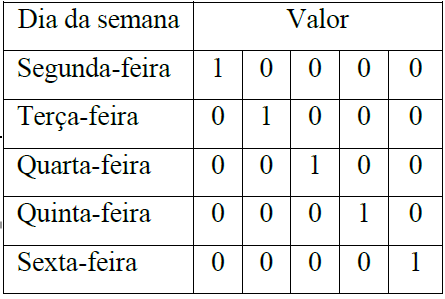
\includegraphics[width=0.65\textwidth]
          		{04-lopes-entradas-dia-semana.png}
          	}
          	\caption{Entradas de dia da semana em cofatores. Retirado de \cite{Lopes2008}.\label{fig:entradasSemanais}}
            \end{figure}

            Os dados estruturados ficarão de acordo com a Tabela 1, onde a coluna $X_i$ receberá os dados da coluna $i+1$ 3ª linha até a 2ª até a 15ª linha, e o valor $Y_i$ receberá o dado da coluna $i+1$ na 1ª linha:
            \begin{table}[!ht]
          	\centering
          		\caption{Tabela de dados do R.U.}	\label{tab:regressaoMultipla}
                  
          				\begin{tabular}{|c|c|c|}
          			\hline \textbf{ }   &\textbf{26/02/2018} &\textbf{27/02/2018}\\
          			\hline \textbf{VENDAS - $Yi$}   &\textbf{446} &\textbf{470}\\
          			\hline \textbf{PARÂMETROS $Xi$}   &\textbf{ } &\textbf{ }\\
          			\hline Temperatura(C)      &27.2 	 			& 28.5\\
          			\hline Precipitação(\%)    & 88         		& 84\\

          			\hline Segunda             & 1          		& 0\\
          			\hline Terça               & 0          		& 1\\
          			\hline Quarta              & 0          		& 0\\
          			\hline Quinta              & 0          		& 0\\
          			\hline Sexta               & 0          		& 0\\

          			\hline Primavera           & 0          		& 0\\
          			\hline Verão               & 1          		& 1\\
          			\hline Outono              & 0          		& 0\\
          			\hline Inverno             & 0          		& 0\\

          			\hline 1o Semestre         & 1          		& 0\\
          			\hline 2o Semestre         & 1          		& 0\\
          		\end{tabular}
            \end{table}
            
            Por fim a partir da tabela, os dados serão separados em forma de matrizes para aplicação nos métodos de regressão linear e aprendizado de máquina, conforme o exemplo abaixo.
            
            $$Y=\left[\begin{array}{c}
            446\\
            470\\
            \end{array}\right]~~
            ~~X=\left[\begin{array}{ccccccccccccc}
            ~27.2 ~88 ~1 ~0 ~0 ~0 ~0 ~0 ~1 ~0 ~0 ~1 ~1\\
            ~28.5 ~84 ~0 ~1 ~0 ~0 ~0 ~0 ~1 ~0 ~0 ~1 ~1\\
            \end{array}\right]$$

      % ----------------------------------------------------------
      % ESTATÍSTICA
      % ----------------------------------------------------------
      \section{Análises Estatísticas}
        \subsection{Análise Exploratória dos Dados}
          \cite{Junior2007} Cita que dados coletados em modelos de previsão possuem informações que quando são projetadas graficamente evidenciam comportamentos que em alguns casos podem ser visualizados e generalizados de forma subjetiva pelos gestores dos dados.  
          Em todos os casos, a análise exploratória é necessária para selecionar o melhor método de análise que se enquadra neste comportamento.

          Somente a análise exploratória não é o suficiente e realizada nos intervalos ou critérios incorretos pode comprometer seriamente as conclusões do comportamento dos dados, e que por sua vez pode comprometer seriamente a decisão dos gestores responsáveis por estes dados, no cenário de uma previsão de demanda. 
          Isto ocorre atualmente no cenário de previsão da demanda de refeições do ICT-UNIFESP, onde a universidade e o estabelecimento que fornece as refeições não tem nenhum modelo de previsão de demanda. 

          De acordo com o gestor da atual empresa que fornece refeições no ICT, a análise utilizada para se prever as refeições é observar dentro da semana o dia anterior de consumo. Em variações de 300 para 450 refeições aproximadamente, isso tem provocado um desperdício médio de 150 refeições diárias. Em geral, de acordo com o restaurante, todos os dias o mesmo trabalha com um erro e um descarte de 30\% das refeições que são trazidas e consumidas ao campus. Estima-se então que no período de 2011 - 01/08/2018 os estabelecimentos tenham tido um prejuízo de R\$1.885.938,40, e de 30\% de R\$78.386,85 no atual período de 01/08/2018 - 31/10/2018 totalizando o montante  R\$1.964.325,25. Aproximadamente 2 milhões de reais em prejuízo acumulado desde 2011.

        \subsection{Métodos de Previsão} 

          \cite{Junior2007} Realiza uma revisão bibliográfica extensa abordando principais métodos de previsão de consumo sazonais, no cenário de uma indústria cosmética. Tais métodos estatísticos de previsão se dividem em 2 ramificações, sendo quantitativos ou qualitativos. Métodos qualitativos fazem um julgamento dos dados expostos sem um sistema de processamento analítico para se produzir novos modelos ou dados, eles são úteis para sistemas de agrupamento, clusterização ou classificação de dados, sem fornecer novas informações numéricas ou modelos preditivos.

          Métodos quantitativos que é o foco deste trabalho, são analíticos e se baseiam em um modelo matemático para realizar previsões. 

          Para realizar tais previsões os métodos quantitativos necessitam de um histórico de dados, para analisar padrões em seu comportamento e predizer o futuro que irá agir dentro deste padrão.

          Estes métodos se ramificam em 2 tipos, as séries temporais e os modelos causais.
          \begin{figure}[!ht]
          	\center{
          		\includegraphics[width=0.65\textwidth]
          		{01-junior-metodos-quantitativos.png}
          	}
          	\caption{Tipos de métodos quantitativos Retirado de \cite{Junior2007}.\label{fig:metodosQuantitativos}}
          \end{figure}

        \subsection{Métodos de previsão de Demanda}
          O autor supracitado também referencia métodos estatísticos especialmente selecionados para uma previsão de demanda, com a atenção de que alguns métodos qualitativos foram criteriosamente selecionados para prever uma demanda industrial, onde geralmente são previstas pelos métodos quantitativos.

          O comportamento dos dados deste trabalho, apesar de ter uma distribuição de datas, que são em função do tempo e se classificando em um modelo de série temporal, assume-se a hipótese que tem tal comportamento impactado por relações causais com outras variáveis como recesso acadêmico, feriados, eventos, precipitações intensas que causam trânsito local e impactam na logística e frequência do público, entre outras variáveis de causas menos aparentes.

          \begin{figure}[!ht]
          	\center{
          		\includegraphics[width=0.65\textwidth]
          		{02-junior-metodos-previsao-demanda.png}
          	}
          	\caption{Métodos de previsão de demanda \cite{Junior2007}.\label{fig:metodosPrevisaoDemanda}}
          \end{figure}

        \subsection{Meta-análise}
          \cite{Flavia2014} cita em sua tese, que resultados e modelos obtidos a partir de análises experimentais em determinado trabalho científico tem a expectativa de confirmação em um padrão de repetição futura, mas que nem sempre tal expectativa é cumprida. Logo é interessante que seja realizado uma análise das análises, ou seja, a comparação de resultados de diferentes métodos obtendo conclusões mais confiáveis e informativas do que o uso único de uma análise.

          Portanto a distribuição de observações de vendas do restaurante universitário, em função do tempo, será tratada como um modelo de relação causal e quantitativo, e conforme a figura 2 será implementado o método estatístico de regressão linear, e os métodos de inteligência artificial de redes neurais, que obteram sucesso nos trabalhos relacionados desta pesquisa, após isso o resultado de ambos serão submetidos à uma meta-análise, e tais métodos serão explicados nos capítulos a se seguir.

        \subsection{Séries Temporais}
          De acordo com  \cite{Morettin1987} uma série temporal é um conjunto de observações ordenadas em função do tempo, comumente iguais, apresentando uma dependência serial entre elas, sendo um dos objetivos do estudo de séries temporais, analisar e modelar essa dependência. Além disso, séries temporais são analisadas pelos seus principais movimentos, como tendência, sazonalidade e a componente aleatória, sendo a tendencia e sazonalidade as propriedades que mais ganham destaque em pesquisas de previsão de demanda de carga elétrica. Os meios mais comuns de se analisar a componente sazonal são o Método de Regressão (paramétrico), Método de Médias Móveis (não paramétrico), e Método de Diferença Sazonal (sazonalidade determinística).  Neste trabalho, a distribuição dos dados do Restaurante se dá de forma paramétrica, ou seja, as vendas do restaurante se distribuem em função do tempo e com influências de parâmetros como o dia da semana por exemplo, sendo ideal as análises de regressão. 

          \cite{Almeida2013} também cita que para realizar a previsão de uma determinada série temporal é possível utilizar diferentes métodos. Pode-se classificá-los basicamente entre métodos estatísticos e baseados em inteligência artificial.
          Dentre os métodos estatísticos destacam-se:
          \begin{itemize}
          \item Regressão Linear Múltipla;
          \item Alisamento Exponencial;
          \item Média Móvel Integrada Auto-Regressiva (ARIMA)
          \end{itemize}
          Entre os métodos baseados em inteligência artificial tem-se:
          \begin{itemize}
          \item Redes Neurais Artificiais;
          \item Lógica Fuzzy.
          \end{itemize}

        \subsection{Componentes Temporais}

          É importante observar que os métodos de previsão em séries temporais buscam uma redução da série temporal à um modelo estacionário e a decomposição da série em componentes de tendência, ciclo, sazonalidade (próxima figura) e termo aleatório. A tendencia se entende pelo movimento persistente dos dados em uma direção, o ciclo indica o movimento oscilatório desta tendência, sazonalidade indica comportamento regular assumido de forma repetitiva e o termo aleatório se dá por movimentos irregulares presentes na série.
           
          As técnicas de previsão para evidências sazonais, conforme  usam métodos de regressão, que pode ser observados nos trabalhos de previsão de consumo de energia elétrica realizados por \cite{Almeida2013}, \cite{RUAS2012}, \cite{Silva2010} e de previsão de demanda de produtos cosméticos em \cite{Junior2007}

          O cenário deste estudo analisa a frequência de alunos dentro do ICT - UNIFESP e consequentemente dentro do R.U tem sazonalidade anual a partir do momento em que a grade de disciplinas tender a ter sazonalidade anual. \\

          \begin{figure}[!ht]
          	\center{
          		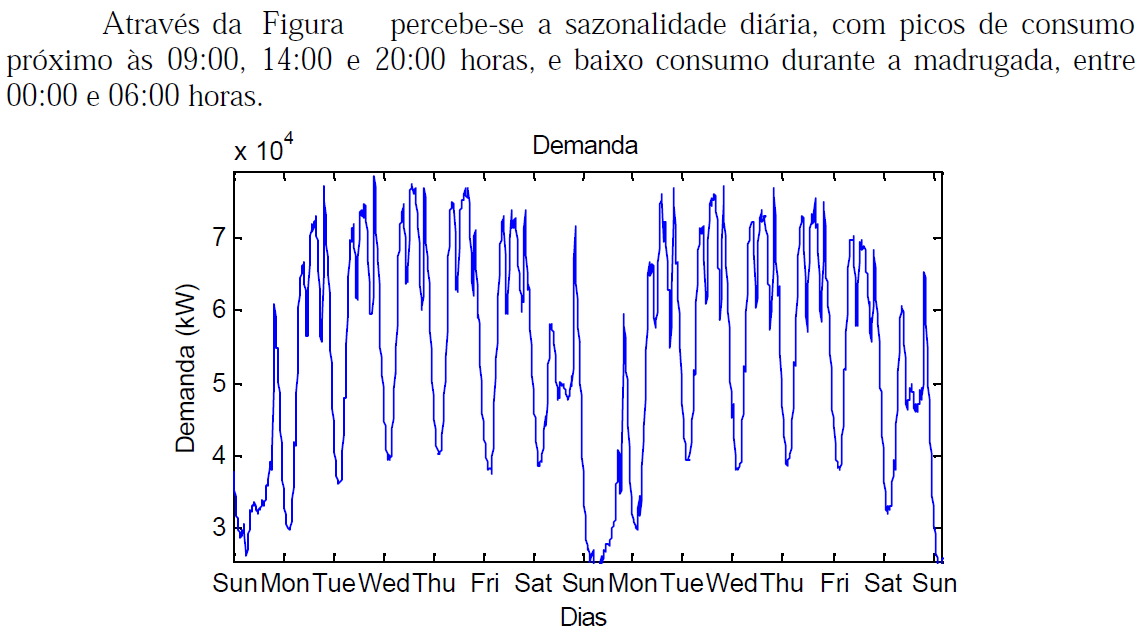
\includegraphics[width=0.65\textwidth]
          		{03-ruas-serie-temporal-sazonal.png}
          	}
          	\caption{DADOS DE DEMANDA DE SAZONALIDADE DIÁRIA, EM FUNÇÃO DO HORÁRIO. Retirado de \cite{RUAS2012}.\label{fig:seriesTemporais}}
          \end{figure}

        \subsection{Previsão com Regressão Linear Múltipla}
          A teoria da regressão se iniciou no século XIX com Galton, que analisou a altura dos pais e dos filhos ($X_i$ e $Y_i$) e buscou a influencia da altura do pai no filho, notando que a altura do filho tendia à media da altura do pai, e chamou esta técnica de regressão pois existe uma tendência dos dados regredirem à média.

          \cite{Clarice2011} Informa que em estudos de regressão aplica-se o método relacionar uma variável aleatória Y com uma variável X, e no caso da regressão múltipla com múltiplas variáveis X, representando causas diferentes que se combinam para a ocorrência de um valor Y. 

          No exemplo abaixo de regressão linear simples, podemos analisar o total de venda Y de um dia X, sendo relacionado nas variações $(\beta_0, \beta_1, ..., \beta_k)$ de datas de $X$.

          Ou seja, $X,Y \rightarrow Y \simeq f(X) $\\
          Na regressão simples $Y$ depende apenas de uma variável $X$, isto é, $Y \simeq f(\beta_0, \beta_1, ..., \beta_k) + E_y$, Sendo $E_y$ um erro aplicado à esta função para se chegar no valor $Y$. Logo a função $f(.)$ pode ser linear nos parâmetros $(\beta_0, \beta_1, ..., \beta_k)$, se a derivada da função em relação às derivadas dos parâmetros, corresponderem à $h(X),i$, para $i$ variando de $0$ à $k$. Sendo $h(X),$ dependente apenas de $X$.
          $\frac {\partial f}{\partial \beta_i} = h (X),i = 0,1,...,k $

          Na regressão múltipla, onde temos múltiplas relações causais $X_1$ à $X_k$, em ocorrências $\beta_0$ à $\beta_k$, temos a função: $Y \simeq f(X_1, X_2, ..., X_k, \beta_0, \beta_1, ..., \beta_k) + E_y$. Também sendo linear nos parâmetros se a derivada da função em relação às múltiplas derivadas dos parâmetros, corresponderem à $h(X_1,X_2,...,X_k)$, tendo $h(.),$ dependente apenas de $X_1,X_2,...,X k$. Em caso contrário, $f(.)$ é uma função não linear dos parâmetros.

          Logo, $Y=f(X_1,X_2,...,X_k,\beta_0,\beta_1,...,\beta_k)+E y$ é linear nos parâmetros se:
          $\frac {\partial f}{\partial \beta_i} = h(X_1,X_2,...,X_k)$
          
          \paragraph{Representação dos dados}
          Na tabela abaixo representa-se a estrutura de dados para regressão linear múltipla, com n observações da variável resposta $Y$ e $p$ variáveis explicativas. Assim, $y_i$ é o valor da i-ésima resposta e $x_{ij}$ na é o valor da variável $x_j$ do conjunto de $j$ variáveis correspondente à resposta $y_i$ .
          Para que seja possível aplicar o método dos quadrados mínimos (explicado adiante) de resolução do sistema de variáveis $X$ em relação à $Y$, é importante que se obtenha p observações $Y$, onde $n\geq (p+1)$.
          
          \begin{table}[!ht]
          	\centering
          		\caption{Representação de dados para regressão múltipla.}	\label{tab:regressaoMultiplaEstrutura}                  
          				\begin{tabular}{|c|c|c|c|c}          			
          				\hline $y$ & $x_1$ & $x_2$ & ... & $x_p$\\
                        \hline $y_1$ & $x_{11}$ & $x_{12}$ & ... & $x_{1p}$\\
                        \hline $y_2$ & $x_{21}$ & $x_{22}$ & ... & $x_{2p}$\\
                        \hline $\vdots$ & $\vdots$ & $\vdots$ & ... & $\vdots$\\
                        \hline $y_n$ & $x_{n1}$ & $x_{2n}$ & ... & $x_{np}$\\
          		\end{tabular}
          \end{table}
          Satisfazendo o modelo final $Y_i = \beta_0 + \beta_1*x_{i1} + \beta_2*x_{i2} + \beta_p*x_{ip} + \epsilon_i$\\
          $i=1,...,n$
          
          \paragraph{Método dos Mínimos Quadrados}
          O método dos mínimos quadrados, é uma técnica utilizada popularmente em estimações econômicas, que busca encontrar o melhor ajuste de um conkunto de ados conforme tabela e modelo acima, para minimizar a soma dos erros quadráticos $\epsilon$. A técnica foi publica por Adrien-Marie Legendre em 1809, em Nouvelles méthodes pour la détermination des orbites des comètes, realizando a hipótese de que a distribuição do $\epsilon$ seja aleatória e normal, embora tal dedução já existisse indiretamente nos teoremas de Gauss-Markov.
          
          A minimização da soma dos erros quadráticos busca então minimizar a seguinte equação $L$:
          
          $L = \sum_{i=1}^{n} \epsilon_i^2 = \sum_{i=1}^{n}(Y_i-\beta_0-\beta_1*x_{i1}-...-\beta_p*x_{ip})^2$
          
           A técnica segue o principio de ser linear nos parâmetros, já demonstrado acima conforme \cite{Clarice2011}.
           Logo deriva-se L em função dos parâmetros $\beta$.\\
           $\frac {\partial L}{\partial \beta_0} = -2 \sum_{i=1}^{n}[Y_i-\beta_0-\beta_1*x_{i1}-...-\beta_p*x_{ip}]$\\
           $\frac {\partial L}{\partial \beta_j} = -2 \sum_{i=1}^{n}[Y_i-\beta_0-\beta_1*x_{i1}-...-\beta_p*x_{ip}]x_{ji}$
          
          Aplicando-se álgebra, igualando as derivadas parciais a zero e organizando o sistema em forma matricial, o modelo final pode ser dado por: $$\begin{equation*}Y=X\beta+\varepsilon,\end{equation*}$$.
          
          $$Y=\left[\begin{array}{c}Y_1\\Y_2\\\vdots\\Y_n\\\end{array} \right]~~,~~X=\left[\begin{array}{ccccc}1~x_{11}~ x_{12}~\ldots~x_{1p}\\1~x_{21}~x_{22}~\ldots~x_{2p}\\\vdots~~~\vdots~~~\vdots~~~\ddots~~~\vdots\\1~x_{n1}~x_{n2}~\ldots~x_{np}\\\end{array} \right]~~,~~\beta=\left[ \begin{array}{c}\beta_0\\\beta_1\\\vdots\\\beta_p\\\end{array} \right]~~\mbox{e}~~ \varepsilon=\left[ \begin{array}{c}\varepsilon_1\\\varepsilon_2\\\vdots\\\varepsilon_n\\\end{array}\right],$$
          
          Logo, $$\frac{\partial L}{\partial\beta}=-2X^\prime Y+2X^\prime X\beta.$$
          
          Aplicando-se álgebra matricial, substituindo o vetor de coeficientes $\beta$ por $\widehat\beta$ que é o objetivo da relação busca entre as variáveis $X$ e $Y$:
          $ \begin{equation*}\widehat{\beta}=(X^\prime X)^{-1} X^\prime Y.\end{equation*} $
          
          Portanto o modelo final é dado por $Y_{estimado} = X\widehat{\beta}$.
          
        \subsection{Algoritmo de Regressão Linear Multipla}
        
            \begin{enumerate}
                  \item Estruturação dos dados em forma matricial, $Y_{1,1...n}$ e $X_{1...n,1...j}$, sendo $n \geq (j+1)$ \\
                  \item Obtenção do vetor de coeficientes $\widehat{\beta}$ das variáveis $X$, através da operação $\widehat{\beta}=(X^\prime X)^{-1} X^\prime Y$
                  \item Construção do modelo final por $Y_{estimado} = X\widehat{\beta}$.
            \end{enumerate}
      % ----------------------------------------------------------
      % INTELIGENCIA ARTIFICIAL
      % ----------------------------------------------------------
      \section{Inteligencia Artificial}
        \paragraph*{A Inteligência artificial} "A inteligência artificial é o ramo da ciência da computação que se ocupa do comportamento inteligente." \cite{Luger2004}.
          O termo "Inteligencia Artificial" surgiu em meados de 1956 em uma conferência, chamada Dartmouth Summer Research Project on Artificial Intelligence, sediada nos Estados Unidos em Dartmouth College, Hanover, New Hampshire, a conferência foi organizada por John McCarthy e teve como proposta reunir matemáticos, cientistas da computação e pesquisadores buscando descbrori como fazer com que as máquinas usem linguagem, abstrações de formulários e conceitos, para resolver problemas que eram reservados aos humanos, e que consigam melhorar o seu próprio desempenho.

          Sistemas de inteligência artificial buscam então resolver funções e problemas que seres humanos conseguem resolver melhor do que máquinas convecionais, usando sua capacidade de abstração e aprendizagem com o erro.

        \subsection{Neuronio Artificial}
         
          \paragraph*{História e inspiração da Inteligência Artificial}
            Redes Neurais Artificiais são elementos de inteligência artificial da ciência da computação, inspirados no funcionamento do cérebro humano.
            São formadas por neuronios artificiais interconectados que são capazes de processar múltiplos valores de entradas, e reagir produzido uma resposta relacionada à essas entradas.
            Como qualquer outro método de aprendizado de máquina, este modelo busca obter um aprendizado a partir dos dados de entrada recebidos, criando uma capacidade de generalização de problemas e assim buscam o objetivo principal de resolver novos problemas com este aprendizado.

            Uma rede neural pode não produzir uma resposta esperada, resolvendo erroneamente um problema, assim como o cérebro humano tem limitações de aprendizado, que levam o homem a cometer falhas de decisões ou ações por um aprendizado mal treinado. Por isso as características fundamentais que tornam uma rede neural artificial em uma boa solução, é um bom planejamento de sua topologia, e método de treinamento, que serão explicados a seguir.

            \cite{Muhammad2014} Demonstra em sua pesquisa que a propriedade fundamental do cérebro é a sua capacidade de mudar com uma grande variedade de experiências, inclusive lesões que provocam perdas de neurônios, abordando princípios de plasticidade cerebral, mostra também que a capacidade de aprendizado de mamíferos que sofreram uma redução de neurônios causada por lesões, pode ser restaurada não somente pela recuperação desses neurônios perdidos, mas sim por novas conexões e sinapses entre outros neurônios. Ou seja, a rede sofre uma mudança de topologia.

            \cite{Fapesp192} Mostra em um experimento recente que o cérebro humano possui atualmente 86 bilhões de neurônios interconectados, e que sua capacidade de aprendizado e habilidades evolutivas também vêm aumentando em conjunto com seu número de neurônios e topologia de rede neural, que há 30 milhões de anos atrás tinha apenas 2,5 bilhões de neurônios e era apenas um animal arborícola quadrúpede.

          \paragraph*{Neuronio Biológico}
            O modelo de neurônio artificial surge então, com a busca da inteligência artificial de reproduzir o comportamento de aprendizado humano, reproduzindo computacionalmente seu elemento biológico principal de aprendizagem: O neurônio biológico. 
            \begin{figure}[!ht]
              \center{
                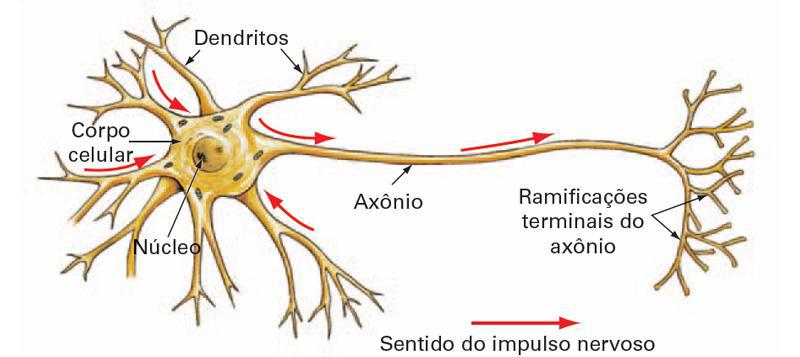
\includegraphics[width=0.65\textwidth]
                {05-neuronio.jpg}
              }
              \caption{Neuronio Biológico, retirado de https://pt.khanacademy.org/science/biology/human-biology/neuron-nervous-system/v/anatomy-of-a-neuron.\label{fig:NeuronioBiológico}}
            \end{figure}
            Um neurônio biológico (Figura 05) processa informações recebidas por meio de seus dentritos e processa-as em seu corpo celular, tal reação à esses estímulos recebidos gera um sínal de saída como resposta aos estímulos, enviado através do axônio. Esse estímulo é repassado como sinal de entrada, através de outros neurônios por meio de seus dendritos, e o ciclo se repete em uma vasta rede.
            Controlando essas conexões, pontos de contato entre a resposta de um neurônio e a entrada de outro, existem as sinapses. Elas funcionam como agentes que permitem a interação acontecer ou inibem, e são acionadas por um conjunto somatório de estímulos. Se tal somatório de estímulos for satisfatório, elas permite a transmissão de sinal elétrico pelo axônio até o dendrito de um neurônio vizinho, formando um ciclo de aprendizado em uma rede neural biológica.

          \paragraph*{Neuronio Artifical}
            Warren McCulloch e Walter Pitts em 1942 observando o neurônio biológico iniciam a busca de um modelo computacional do mesmo. McCuloch era psiquiatra e neuroanatomista e passou cerca de 20 anos refletindo e estudando sobre a representação do sistema nervoso, em 1942 ele convidou Pitts, que era matemático, para fazer parte das suas pesquisas.Em 1943 lançaram o artigo "A Logical Calculus of the Ideas Immanent in Nervous Activity." chegando em um modelo matemático do neurônio artificial: 

            \begin{figure}[!ht]
                \center{
                  \includegraphics[width=0.65\textwidth]
                  {06-neuronio-artificial.png}
                }
                \caption{Neuronio Artificial\label{fig:NeuronioArtificial}}
            \end{figure}

            Assim como no neurônio biológico, este modelo reage à um vetor de entradas $X0,X1,...,Xn$ onde tem suas sinpases representadas por pesos numéricos, existe uma soma ponderada dessas entradas que é controlada por uma função de transferência ou função de ativação, determinando se essa soma é maior que um valor numérico. Se essa soma for satisfatória o neurônio é ativado emitindo um valor de saída 1, caso contrário se emite um valor de saída 0.
            Todo o funcionamento deste modelo então é reduzido a responder se a soma recebida é maior que um valor numérico esperado.

            Neste modelo simplista o neurônio consegue realizar operações lógicas. Na figura 07 os pesos w1 e w2 e o limiar T estão ajustados para responder à operação AND que resumidamente é uma operação lógica que somente produz um valor positivo 1 na resposta de saída se ambos os valores de entrada forem 1.

            \begin{figure}[!ht]
              \center{
                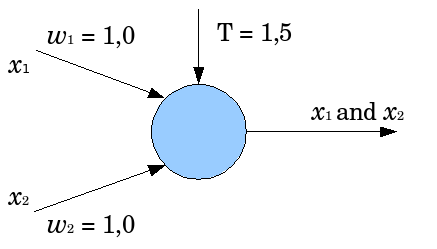
\includegraphics[width=0.65\textwidth]
                {07-neuronio-operacao-and.png}
              }
              \caption{Neuronio Artificial - Operação AND\label{fig:NeuronioArtificialAnd}}
            \end{figure}

            Neste modelo o neurônio irá comparar se a soma das entradas $X$ multiplicadas pelos seus devidos pesos $W$, será menor que o limiar T. Ele somente irá produzir uma resposta positiva (1) se essa soma for maior. É fácil verificar então na imagem, que o resultado dessa soma só será positivo, se ambas as entradas forem 1, onde a soma será $2>1,5$.

            \begin{table}[!ht]
            \centering
            \caption{Operação Lógica AND} \label{tab:and}
              \begin{tabular}{|c|c|c|}
                  \hline  \textbf{A} & \textbf{B} &  \textbf{Saída}\\
                  \hline 0 & 0 & 0\\
                  \hline 0 & 1 & 0\\
                  \hline 1 & 0 & 0\\
                  \hline 1 & 1 & 1\\
                  \hline 
              \end{tabular}
            \end{table}

        \subsection{Redes Neurais Artificiais}
          \paragraph*{Perceptron}
            O modelo de Warren McCulloch e Walter Pitts, apesar de conseguir simular o modelo de neurônio biológico e resolver algumas tarefas lógicas e matemáticas não atendia o objetivo principal da Inteligência Artificial: A capacidade de aprendizado.
            Para utilizar um modelo de neurônio artificial a fim da solução de um problema era necessário conhecer o ajuste dos pesos das entradas, e em uma tarefa de um cenário complexo e com muitas variáveis, ou pesos não perceptíveis ao valor esperado de saída, este ajuste não se torna trivial.
            
            Em 1958, o cientista da computação Frank Rosemblatt desenvolveu o modelo de neurônio artificial Perceptron para solucionar este problema de ajuste de pesos.
            Basicamente neste novo modelo, os pesos das conexões são ajustados de forma autônoma com a introdução de pessoas associados e uma valor bias, a fim de buscar um reconhecimento autônomo de padrões. Tarefas de reconhecimento de padrões simples com separações lineares os seres humanos conseguem realizar de forma trivial mas ainda era um desafio para tal problema se resolvido por uma máquina.

            O perceptron \cite{Flavia2014} possui apenas uma camada de entrada e saída, a saída utiliza como função de ativação a função degrau $u$ que define quando o neurônio emitirá o sinal lógico 1 ou quando emitirá o sinal lógico 0.

            O sinal de saída do perceptron entende-se então por:
            $y= \delta(\sum_{i=1}^{n}XiWi+b)$
            \begin{itemize}
            	\item $ Xi $ - sinais de entrada do neurônio;
            	\item $ Wi $ - pesos sinápticos do neurônio;
            	\item $ b $ - bias ou limiar de ativação;
            	\item $ \delta(.) $ - função de ativação;
            	\item $ y $ - sinal de saída do neurônio.
            \end{itemize}
			
            \begin{figure}[!ht]
            	\center{
              \includegraphics[width=0.65\textwidth]
              {08-perceptron.png}
            }
            \caption{Neuronio Artificial Perceptron\label{fig:perceptron}}
            \end{figure}
			
			     Em algumas literaturas o bias pode ser reduzido a um peso $W0$ com entrada $X0$ fixo em 1 no neurônio, a representação gráfica da topologia pode mudar, mas no somatório de saída, o calculo continua o mesmo.
			
			     A função de ativação $\delta$ se apresenta de forma linear ou não linear, determinando a saída de um neurônio a partir do seu potencial de ativação. 
			     As funções de ativação podem ser observadas na figura 09, sendo a de maior popularidade de utilização, a sigmoide.
			
			     \begin{figure}[!ht]
    				\center{
    					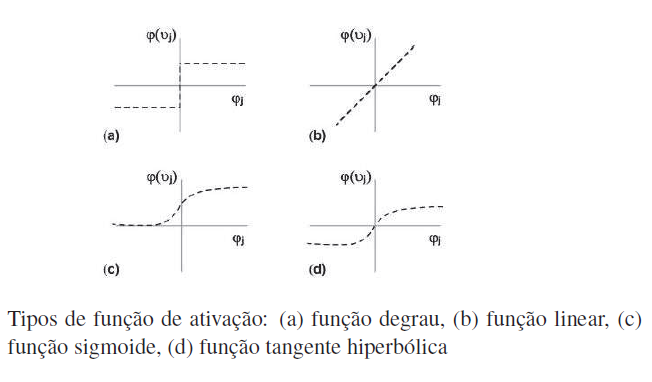
\includegraphics[width=0.65\textwidth]
    					{09-delta.png}
    				}
    				\caption{Funções de Ativação retirado de \cite{Flavia2014} \label{fig:perceptron}}
			     \end{figure}
			
				    As funções de ativação dá a capacidade do perceptron quando conectado em rede (explicado no próximo capítulo) de resolver problemas lineares e não lineares, agregando adaptação e improviso ao resolver programas que não estão contidos em seus dados de alimentação.
			
		      \paragraph*{Perceptron - Treino Supervisionado}
            \cite{Almeida2013} cita que o processo de aprendizado do perceptron pode ocorrer de forma supervisionada quando o neurônio deve aprender a relacionar um conjunto observado de variáveis à um valor observado de saída deste mesmo conjunto. O neurônio recebe os sinais de entrada $Xi$ e produz uma saída $Yi$ através do combinador linear e função $\delta$ de ativação; compara essa saída $Yi$ com a observação $i$ obtida do conjunto de dados (ponto chave do processo de treino supervisionado) e por fim essa comparação irá gerar um erro $e$.
            
            \subparagraph* {Critério de parada}
            	De acordo com algum critério adotado em cada contexto de aplicação do perceptron, este erro pode ser aceitado e o neurônio mantém o valor de seus pesos $Wi$ que impactam na saída $Yi$ desejada. A aprendizagem do neurônio também pode atingir um critério de parada após N épocas de treinamento, diversos critérios de paradas  podem ser combinados.  
            	
            \subparagraph* {Época de treinamento}
            	Se o critério de parada não for aprovado, uma nova época de treinamento (ou repetição de interação) é iniciada mesmos valores $X_i$ e $Y_i$ passados, os valores de pesos $Wi$ são reajustados com a taxa de aprendizagem, buscando o objetivo de se obter um erro menor.
            	
            \subparagraph* {Taxa de aprendizagem}
            	Esse reajuste de pesos $Wi$ denomina-se taxa de aprendizagem, $\alpha$ que pode ter valores de escolha livre ao contexto de aplicação do perceptron, para reajustar estes pesos $Wi$. Assim que a taxa de aprendizagem ajusta os pesos, uma nova época N+1 de treinamento está se iniciando buscando novamente um erro menor. Ressaltando então que o critério de parada pode ser acionado e interromper o reinicio do processo, se for estipulado um limite para o valor de N combinado ou não com um limite para o erro. 
            	
          \subsection {Funcionamento e treino do neurônio perceptron}
            Em \cite{Almeida2013} verifica-se de forma procedural, o processo do treino supervisionado do perceptron, com $m$ observações $Y$ = $(Y_{i},Y_{i+1}...,Y_{m})$ com $n$ entradas $X$ relacionadas à cada $Y_m$, ocorre da seguinte maneira: 
            Matematicamente o neurônio é representado por um vetor global de $n$ pesos sinápticos $(W_0, W_{1}, ..., W{n})$ , e um valor de bias $b$. O processo do algoritmo abaixo ajustará esses pesos e bias.
            \begin{enumerate}
              \item Coleta do valor supervisionado inicial $Y_{0}$, que é a primeira observação histórica do conjunto de dados.
              \item Coleta do vetor de variáveis $(X_{00}, X_{01}, ..., X_{0n})$ relacionados à saída supervisionada $Y_i$.
              \item Inicialização dos pesos sinápticos $(W_0, W_{1}, ..., W{n})$ com valores aleatoriamente pequenos.
              \item Definição de um valor real entre 0 e 1 para a taxa de aprendizado $\alpha$.
              \item Definição do valor inicial de bias $b$.
              \item Definição da função de ativação $\delta$ 
              \item Definição do limite de épocas de treino $l_e$, se não houver, definir $l_e$ para -1.
              \item LAÇO: Percorrer e atribuir em ($Y_d$) de $Y_0$ até $Y_m$, inicializando o contador de épocas $c_e$ = 0, enquanto $CP(e)$ for verdadeiro E/OU ($l_e$) for menor que $c_e$:
              \item Nova coleta do vetor de variáveis $(X_{d0}, X_{d1}, ..., X_{dn})$ relacionados à saída supervisionada $Y_d$.
              \item Incrementar 1 em $c_e$.
              \item Cálculo do sinal $u = \sum_{i=1}^{n}X_{di}*W_{i}+b$
              \item Aplicação de valor de $U$ na função de ativação $\delta$ obtendo $Y_u = \delta(u)$
              \item Obtenção do erro $e = Y_d-Y_u$
              \item Aplicação do critério de parada $CP$ em relação ao erro $e$; $CP(e)$
              \item SE $CP(e)$ for APROVADO, o algoritmo continua, SE REPROVADO, a aprendizagem é feita ajustando $b_{}=b_{}+(\alpha*(e))$, e ajustando o vetor $W_{i} = W_{i}+(\alpha*e*X_{di})$. 
            \end{enumerate}
 
        \paragraph* {Funcionamento do perceptron para logica AND}.\\
		 Este exemplo aborda a aplicação do problema do neurônio de Warren McCulloch e Walter Pitts, o aprendizado para a tabela AND, que busca fornecer uma resposta verdadeira apenas se a primeira E todas as demais entradas forem verdadeiras.\\            	
        A utilização do perceptron com o modelo de aprendizado supervisionado, busca então conseguir de forma autônoma os valores de pesos $W_i$ e desta forma aprender o funcionamento da logica E, sem que seja necessário a tarefa humana de ajustar o mesmo.\\
                 \begin{table}[!ht]
                 \centering
  				  \begin{tabular}{|c|c|c|c|}
  				 	\hline  \textbf{linha} & \textbf{$X_0$} & \textbf{$X_1$} &  \textbf{$Y$}\\
  				 	\hline 0 & 0 & 0 & 0\\
  				 	\hline 1 & 0 & 1 & 0\\
  				 	\hline 2 & 1 & 0 & 0\\
  				 	\hline 3 & 1 & 1 & 1\\
  				  \end{tabular}
                \end{table}
					
  Para este aprendizado vamos definir o critério de parada de 0 para o erro. 
  Definir o valor 0 para o $bias$. 
  1 para $\alpha$ e 
  função $\delta(u)$ = $degrau$ (1, se $u>=0$, 0 se $u<0$).
  O número de épocas terá o mesmo número de valores supervisionado, então o treino executará 1 vez para cada observação.
  			 	   
  			 	 linha $d$ = 0
	  			 \begin{enumerate}
	  			    
	  			 	\item Coleta do valor supervisionado $Y_d$ = $Y_0$ = 0.
	  			 	\item Coleta do vetor de variáveis $(X_{00} = 0, X{01}=0)$.
	  			 	\item Inicialização dos todos os pesos com valores aleatoriamente pequenos: $W_0=3,W_1=3$
	  			 	\item Definição da taxa de aprendizado $\alpha = 1$.
	  			 	\item Definição do valor de bias $b=3$.
	  			 	\item Definição da função de ativação $\delta = degrau$  
	  			 	\item Cálculo do sinal $u = x_{00}*w_0 + x_{01}*w_1 +b = (0*3+0*3+0) = 0$
	  			 	\item Aplicação de valor de $u$ na função de ativação $\delta$ obtendo $Y_u$, $Y_u = \delta(0) = 1$
	  			 	\item Obtenção do erro $e = Y_0-Y_u = 0 - 1 = -1$
	  			 	\item Aplicação do critério de parada $CP$ em relação ao erro $e$ REPROVADO, pois o erro esperado é 0.
	  			 	\item Como $CP$ foi reprovado, a aprendizagem é realizada $b=b+(\alpha*e)$ e $W_i=W_i + (\alpha*e)*X_{0i}$
	  			 \end{enumerate}		
  				
    				Aprendizagem:
    				\begin{enumerate}
    					\item $b=b+(\alpha*e) = 0 + 1*(-1) = -1 $  					
    					\item $W_0=W_0 + (\alpha*e)*X_{00} = 3 + 1*(-1)*0 = 3$
    					\item $W_1=W_1 + (\alpha*e)*X_{01} = 3 + 1*(-1)*0 = 3$
    				\end{enumerate}	
    				
    				Reinicio dos pesos reajustados pela aprendizagem e apresentação da próxima linha ao neurônio:
    				linha $d$ = 1.\\
    				\begin{table}[!ht]
                    \centering
    				\begin{tabular}{|c|c|c|c|}
    					\hline  \textbf{linha} & \textbf{$X_0$} & \textbf{$X_1$} &  \textbf{$Y$}\\
  				 	    \hline 1 & 0 & 1 & 0\\
    				\end{tabular}
    				\end{table}
    				
    				
    				\begin{enumerate}
    				    \item Coleta do valor supervisionado $Y_d$ = $Y_1$ = 0.
    					\item Cálculo do sinal $u = X_{10}*w_0 + X_{10}*W_1 +b = (0*3 + 1*3 -1) = 0$
    					\item Aplicação de valor de $u$ na função de ativação $\delta$ obtendo $Y_u$, $Y_u = \delta(0) = 1$
    					\item Obtenção do erro $e = Y_d-Y_u = 0 - 1 = -1$
    					\item Aplicação do critério de parada $CP$ em relação ao erro $e$ reprovado, pois o erro esperado é 0.
    					\item Como $CP$ foi reprovado, a aprendizagem é realizada $b=b+(\alpha*e)$ e $W_i=W_i + (\alpha*e)*X_{1i}$
    				\end{enumerate}
    				
    				Aprendizagem:
    				\begin{enumerate}
    					\item $b=b+(\alpha*e) = -1 + 1*(-1) = -2 $  					
    					\item $W_0=W_0 + (\alpha*e)*X_{10} = 3 + 1*(-1)*0 = 3$ 
    					\item $W_1=W_1 + (\alpha*e)*X_{11} = 3 + 1*(-1)*1 = 2$
    				\end{enumerate}
    				
    				Reinicio dos pesos reajustados pela aprendizagem e apresentação da próxima linha ao neurônio:
    				linha $d$ = 2\\
    				\begin{table}[!ht]
                    \centering
    				\begin{tabular}{|c|c|c|c|}
    					\hline  \textbf{linha} & \textbf{$X_0$} & \textbf{$X_1$} &  \textbf{$Y$}\\
  				 	    \hline 2 & 1 & 0 & 0\\
    				\end{tabular}
    				\end{table}
            	
            	
            	\begin{enumerate}
            	    \item Coleta do valor supervisionado $Y_d$ = $Y_2$ = 0.
            		\item Cálculo do sinal $u = X_{20}*w_0 + X_{20}*W_1 +b = (1*3 + 0*2 -2) = 1$
            		\item Aplicação de valor de $u$ na função de ativação $\delta$ obtendo $Y_u$, $Y_u = \delta(1) = 1$
            		\item Obtenção do erro $e = Y_d-Y_u = 0 - 1 = -1$
            		\item Aplicação do critério de parada $CP$ em relação ao erro $e$ reprovado, pois o erro esperado é 0.
    				\item Como $CP$ foi reprovado, a aprendizagem é realizada $b=b+(\alpha*e)$ e $W_i=W_i + (\alpha*e)*X_{2i}$
            	\end{enumerate}
            
            	
            	Aprendizagem:
            	\begin{enumerate}
            		\item $b=b+(\alpha*e) = -2 + 1*(-1) = -3 $  					
            		\item $W_0=W_0 + (\alpha*e)*X_{20} = 3 + 1*(-1)*1 = 2$ 
            		\item $W_1=W_1 + (\alpha*e)*X_{21}= 2 + 1*(-1)*0 = 2$
            	\end{enumerate}	
            	
            	Reinicio dos pesos reajustados pela aprendizagem e apresentação da próxima linha ao neurônio:
    				linha $d$ = 3\\
    				\begin{table}[!ht]
                    \centering
    				\begin{tabular}{|c|c|c|c|}
    					\hline  \textbf{linha} & \textbf{$X_0$} & \textbf{$X_1$} &  \textbf{$Y$}\\
  				 	    \hline 3 & 1 & 1 & 1\\
    				\end{tabular}
    				\end{table}
            	
            	\begin{enumerate}
            	    \item Coleta do valor supervisionado $Y_d$ = $Y_3$ = 1.
            		\item Cálculo do sinal $u = X_{30}*w_0 + X_{30}*W_1 +b = (1*2 + 1*2 -3) = 1$
            		\item Aplicação de valor de $u$ na função de ativação $\delta$ obtendo $Y_d$, $Y_u = \delta(1) = 1$
            		\item Obtenção do erro $e = Y_d-Y_u = 1 - 1 = 0$
            		\item Aplicação do critério de parada $CP$ em relação ao erro $e_n$ APROVADO, então conclui-se que os pesos sinápticos estão corretos.
            	\end{enumerate}
                
            	Pesos finais e bias aprovados pelo processo de treino:
            	\begin{enumerate}
            		\item $b=  -3$  					
            		\item $W_1= 2$ 
            		\item $W_2= 2$
            	\end{enumerate}	
            	
            	Fim do processo de treino.
            
            \subparagraph* {Validação do treino}
            	Após todo o processo de treino e apresentação dos conjuntos, é necessário realizar um novo ciclo no perceptron, para ver se o neurônio responde corretamente ao modelo de dados inicial.
            	
            	Pesos finais e bias aprovados pelo processo de treino:
            	\begin{enumerate}
            		\item $b=  -3$  					
            		\item $W_1= 2$ 
            		\item $W_2= 2$
            	\end{enumerate}
            	
                linha $d$ = 0\\
                    \begin{table}[!ht]
                    \centering
    				\begin{tabular}{|c|c|c|c|}
    					\hline  \textbf{linha} & \textbf{$X_0$} & \textbf{$X_1$} &  \textbf{$Y$}\\
  				 	    \hline 0 & 0 & 0 & 0\\
    				\end{tabular}
    				\end{table}
    				
            	\begin{enumerate}
            	    \item Coleta do valor supervisionado $Y_d$ = $Y_0$ = 0.
            		\item Cálculo do sinal $u = X_{00}*w_0 + X_{01}*W_1 +b = (0*2 + 0*2 -3) = -3$
            		\item Aplicação de valor de $U$ na função de ativação $\delta$ obtendo $Y_u$, $Y_u = \delta(-3) = 0$
            		\item Obtenção do erro $e = Y_i-Y_u = 0 - 0 = 0$
            		\item Aplicação do critério de parada $CP$ em relação ao erro $e$ APROVADO, então o neurônio respondeu corretamente às entradas.
            	\end{enumerate}
            	
                linha $d$ = 1\\
                    \begin{table}[!ht]
                    \centering
    				\begin{tabular}{|c|c|c|c|}
    					\hline  \textbf{linha d} & \textbf{$X_0$} & \textbf{$X_1$} &  \textbf{$Y$}\\
  				 	    \hline 1 & 0 & 1 & 0\\
    				\end{tabular}
    				\end{table}
    				
            	\begin{enumerate}
            	    \item Coleta do valor supervisionado $Y_d$ = $Y_1$ = 0.
            		\item Cálculo do sinal $u = X_{10}*w_0 + X_{11}*W_1 +b  = (0*2 + 1*2 -3) = -1$
            		\item Aplicação de valor de $u$ na função de ativação $\delta$ obtendo $Y_u$, $Y_u = \delta(-1) = 0$
            		\item Obtenção do erro $e = Y_d-Y_u = 0 - 0 = 0$
            		\item Aplicação do critério de parada $CP$ em relação ao erro $e$ APROVADO, então o neurônio respondeu corretamente às entradas.
            	\end{enumerate}
            
            	linha $d$ = 2\\
            	    \begin{table}[!ht]
                    \centering
    				\begin{tabular}{|c|c|c|c|}
    					\hline  \textbf{linha d} & \textbf{$X_0$} & \textbf{$X_1$} &  \textbf{$Y$}\\
  				 	    \hline 2 & 1 & 0 & 0\\
    				\end{tabular}
    				\end{table}
    				
            	\begin{enumerate}
            	    \item Coleta do valor supervisionado $Y_d$ = $Y_2$ = 0.
            		\item Cálculo do sinal $u = X_{20}*w_0 + X_{21}*W_1 +b  = (1*2 + 0*2 -3) = -1$
            		\item Aplicação de valor de $u$ na função de ativação $\delta$ obtendo $Y_u$, $Y_u = \delta(-1) = 0$
            		\item Obtenção do erro $e = Y_d-Y_u = 0 - 0 = 0$
            		\item Aplicação do critério de parada $CP$ em relação ao erro $e$ APROVADO, então o neurônio respondeu corretamente às entradas.
            	\end{enumerate}
            
            	linha $d$ = 3\\
            	    \begin{table}[!ht]
                    \centering
    				\begin{tabular}{|c|c|c|c|}
    					\hline  \textbf{linha d} & \textbf{$X_0$} & \textbf{$X_1$} &  \textbf{$Y$}\\
  				 	    \hline 3 & 1 & 1 & 1\\
    				\end{tabular}
    				\end{table}
    				
            	\begin{enumerate}
            	    \item Coleta do valor supervisionado $Y_d$ = $Y_3$ = 0.
            		\item Cálculo do sinal $u = X_{30}*w_0 + X_{31}*W_1 +b  = (1*2 + 1*2 -3) = 1$
            		\item Aplicação de valor de $u$ na função de ativação $\delta$ obtendo $Y_u$, $Y_u = \delta(1) = 1$
            		\item Obtenção do erro $e = Y_d-Y_u = 1 - 1 = 0$
            		\item Aplicação do critério de parada $CP$ em relação ao erro $e$ APROVADO, então o neurônio respondeu corretamente às entradas.
            	\end{enumerate}
           
           		Como o neurônio não teve nenhum critério de parada REPROVADO em todas as interações de todas as linhas, podemos dizer que o mesmo está devidamente treinado e validado para a solução do problema.
            
        \subsection{Limite de um Perceptron}
          É possível reparar que o processo de aprendizagem de um perceptron, se forma por uma combinação linear que é o valor $ u $ dos pesos e entradas xi. Essa combinação pode ser aprovada ou reprovadas no processo repetitivo de treino controlado pela função $\delta$, e pela aprovação do erro medido entre o valor da combinação linear e o valor esperado.
          
          Então em 1969, Marvin Mjinsky e Seymour Papert realizaram uma publicação comprovando essa limitação de aprendizado à uma combinação linear, e provaram que o perceptron é limitado à resolução de problemas que são resolvidos ou classificados por apenas 1 linha, ou seja, problemas linearmente separáveis que consiste na mesma limitação do processo de regressão linear múltipla.
          Na figura 10, abaixo, o perceptron não pode solucionar o problema (b). E essa limitação desmotivou e parou os estudos com perceptrons.
    		  \begin{figure}[!ht]
    		  	\center{
    		  		\includegraphics[width=0.65\textwidth]
    		  		{10-limite-perceptron.png}
    		  	}
    		  	\caption{Problemas Linearmente Separáveis e Não Separáveis. Retirado de \cite{Flavia2014}.\label{fig:problemasLineares}}
    		  \end{figure}
	  	
	  	 Em 1986 James McClelland e David Rumelhart proporam o método de desenvolvimento de uma rede neural de perceptrons, tangindo mais ainda a inspiração da solução no cérebro humano. O processo resume o treinamento do perceptron simples aplicado à um conjunto de perceptrons interligados, e assim solucionando problemas complexos que podem ser resolvidos com uma combinação de soluções.
	  	  
  	  	  \begin{figure}[!ht]
  	  	  	\center{
  	  	  		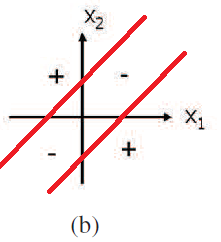
\includegraphics[width=0.30\textwidth]
  	  	  		{11-solucao-mlp.png}
  	  	  	}
  	  	  \caption{Problemas Linearmente Não Separáveis Multiplas Soluções. \label{fig:doisPerceptrons}}
  	  	   \end{figure}
  	    %%%%%%%%%%%%%%%%%%%%%%%%%%%%%%%%%%%%%%%%%%%%%%%%%%%%%   
  	    \subsection{Rede Perceptrons Múltiplas Camadas - MLP}
  	       
  	       A solução base para se combinar 2 ou mais perceptrons a fim de se resolver um problema com a combinação de 2 ou mais soluções lineares, é a utilização de um perceptron combinador de sinal de saída, já que cada perceptron pode ter múltiplas entradas e somente uma saída. Dessa forma as redes neurais vão formando colunas de perceptrons interconectados. Cada coluna é denominada uma camada da rede neural. A ultima camada deve ter o número de perceptrons correspondente ao número de saídas desejadas. Na figura abaixo, encontra-se uma rede neural com duas camadas intermediárias e 3 saídas.
  	       
  	       \begin{figure}[!ht]
  	       	\center{
  	       		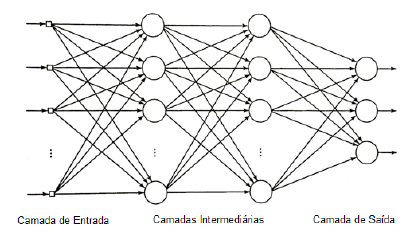
\includegraphics[width=0.65\textwidth]
  	       		{12-mlp.png}
  	       	}
  	       	\caption{Rede de perceptrons com múltiplas camadas. Retirado de \cite{Almeida2013}\label{fig:MLP}}
  	       \end{figure}
         
  	       Esta rede denominada MLP (Multilayer Perceptron) possui uma camada de entrada onde cada nó representa uma variável a ser considerada ao problema a ser analisado, e pelo menos uma camada intermediária.
  	      
  	       Nesta camada intermediária os neurônios possuem geralmente uma função de ativação sigmoidal logística ou tangente hiperbólica, e conceitualmente no mínimo 1 neurônio desta primeira camada oculta deve receber no mínimo 2 conexões de entrada. E uma camada de saída, na borda à direita, com o número de neurônios correspondente ao número de soluções buscadas. 
  	       
            \paragraph{Treino e Validação da MLP}
            	O conjunto de dados de entrada na rede MLP supervisionada, deve ser dividido em 2 partes principais, Treinamento e Validação. É importante salientar que as observações de ambos os conjuntos devem originar do mesmo conjunto de dados para representar o mesmo problema, as observações $Y_i$ relacionadas aos vetores $i$ de variáveis $X_{i1},Xi_{i2},...,X{ij}$ do conjunto de treino, devem ter a mesma estrutura, mesmo número j de variáveis X por vetor de entrada e devem representar o mesmo problema que as observações $Yi$ do conjunto de validação.
            	
            	O conjunto de dados da validação e treino somados devem formar exatamente o conjunto original, sem informações excedentes ou em falta.
            	
            	Os dados de treino e dados de validação, podem ser separados de forma aleatória, sendo os dados de treino os responsáveis pelos reajustes de pesos e capacidade de generalização da rede, e os dados de validação responsáveis pelo processo de validação pós-treino.
            	
            	É importante adotar um bom critério de parada de treino, pois um treino prolongado tende a convergir em ajustes de pesos memorizados dos valores observados nos dados de treino e isso causa o fenômeno de overfitting na rede neural, que é a perda da capacidade de generalização. Pesos sinápticos que sofrem processo prolongado de reajustes acaba "viciando" a rede neural para reconhecer apenas os dados de treino.
            	
            	Parada do erro mínimo:
            	O critério de parada do erro mínimo encerra o treinamento da RNA quando a mesma obtem um erro menor que o mínimo estipulado para o valor observado, este é o critério mais simples, adotado nos casos onde existe um limiar de erro já determinado pelo problema, entre o valor observado e o valor a se predizer.
            	
            	Parada por número de épocas:
            	Um critério de parada pode ser limitado também ao número de épocas de treino. A determinação  deste número de épocas pode ocorrer por tentativa e erro, visto que haverá a convergência de um número pequeno para uma baixa capacidade de aprendizado, e a convergência de um número grande para o processo de overfitting. Logo é necessário realizar experimentos que validem número de épocas fora desses intervalos de convergência.
            	
            	Parada por validação cruzada:
            	Por fim a validação cruzada é a tecnica que se utiliza os dados dos conjuntos de validação e treino de forma cruzada, neste processo então, os dados de treino são utilizados no processo interativo de aprendizagem, e no fim deste processo o conjunto é validado com os dados de validação, obtendo-se um novo erro de validação.
            	A medição do erro de validação passa por um processo de avaliação em função do número de épocas, a fim de se detectar um ponto de número de épocas onde o erro quadrático médio da amostra de validação sofre uma curva de crescimento após um limiar de decréscimo.
            	
            	É notório observar que o erro quadrático médio das amostras de treinamento sofrerá um decréscimo em função do aumento do número de épocas de treinamento, convergindo ao processo de overfitting, ou memorização da rede.
            	
            	O ponto de parada no limite inferior do erro quadrático médio da amostra de validação, será o ponto ótimo de parada de treinamento.
          	
          	\begin{figure}[!ht]
          		\center{
          			\includegraphics[width=0.65\textwidth]
          			{14-validacaocruzada.png}
          		}
          		\caption{Ponto ótimo de parada da validação cruzada. Retirado de \cite{Flavia2014} \label{fig:validacaoCruzada}}
          	\end{figure}
        
        O treinamento de uma rede MLP para previsões de demanda de restaurantes universitários que obteve sucesso em \cite{Lopes2008} e \cite{Rocha2011} é a retro propagação de erro.
        %%%%%%%%%%%%%%%%%%%%%%%%%%%%%%%%%%%%%%%%%%%%%%%%%%%%%%%%%%%%%%%%%%%%%%%
        \subsection{Perceptrons Múltiplas Camadas com Retro Propagação de Erro}
        A rede Perceptron Múltiplas Camadas com Retro Propagação de Erro (do inglês, M.L.P Backpropagation), faz o reajuste dos pesos sinápticos dos neurônios através de duas fases:
  	       \paragraph{Feed-forward} Nesta primeira fase de treino os sinais $X_{i0},X_{i0},...,X_{in}$ com sua respectiva saída $Y_i$ do conjunto de dados são apresentados à todos os neurônios da primeira camada. O processo de propagação do sinal de saída de cada neurônio segue o princípio do neurônio artificial apresentado na seção anterior, que envia o sinal de saída como um sinal de entrada ao neurônio seguinte.
  	       
  	       \paragraph{Feed-backward} Nesta fase é obtido um valor de erro da camada de saída. Este erro é utilizado na equação de reajuste do peso sináptico das conexões dos neurônios da camada de saída com o sinal de saída dos neurônios da última camada oculta. E depois este erro é propagado realizando outra equação de reajuste de peso sináptico das conexões dos neurônios nas camadas anteriores, no sentido contrário em direção à camada de entrada. Isto permite que os pesos sináptico de todas as camadas de intermediárias neste processo tenham seus pesos ajustados.
  	       
  	       \begin{figure}[!ht]
  	       	\center{
  	       		\includegraphics[width=0.65\textwidth]
  	       		{13-mlp-back.png}
  	       	}
  	       	\caption{Fases de treino da MLP-Back-Propagation. Retirado de \cite{Almeida2013}\label{fig:MLP}}
  	       \end{figure}
  	       
  	       \paragraph*{MLP Backpropagation em R.U em trabalhos relacionados}
  	       Em \cite{Lopes2008} A rede neural perceptron de múltiplas camadas é utilizada para tratar a previsão de demanda do R.U da UFV, utilizando apenas como variáveis quantitativas as 5 ultimas observações anteriores ao dia a se analisar, e como variáveis qualitativas o dia da semana variando de segunda a sexta, em valores binários.
  	       
           \begin{figure}[!ht]
          	\center{
          		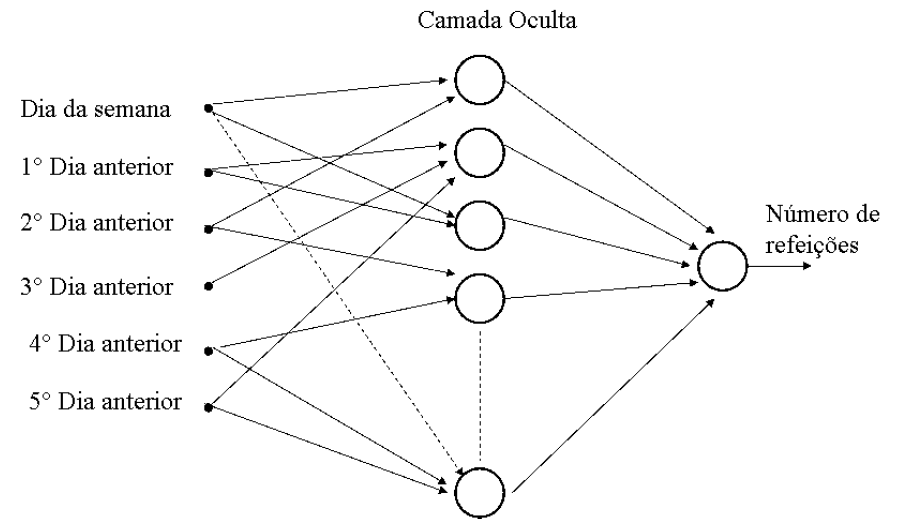
\includegraphics[width=0.65\textwidth]
          		{15-rna-lopes.png}
          	}
          	\caption{Rede Neural Perceptron de Múltiplas Camadas. Retirado de \cite{Lopes2008}.\label{fig:Rna-Perceptron-MultiLayer}}
           \end{figure}
            
           Em \cite{Rocha2011} o trabalho realizado com neurônios artificiais para prever a demanda do R.U da UNESP, envolve apenas uma única camada de entrada e uma segunda camada para saída, porém com uma diversidade maior de variáveis de entrada correlacionadas com o consumo do restaurante. 
           \begin{figure}[!ht]
          	\center{
          		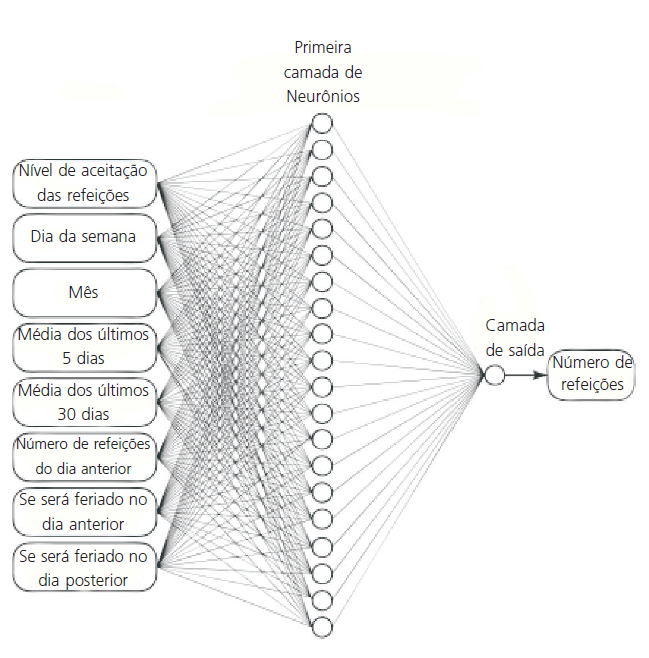
\includegraphics[width=0.65\textwidth]
          		{16-rna-rocha.png}
          	}
          	\caption{Rede Neural Perceptron de Múltiplas Camadas. Retirado de  \cite{Rocha2011} \label{fig:rnaRocha}}
           \end{figure}
         
            Ambos os modelos possuem topologia de uma camada oculta para entrada dos dados, e uma camada de saída. que de acordo com \cite{Braga2000} cita que através de uma análise de Cybenko, uma camada intermediária é o suficiente para aproximar qualquer função contínua e 2 camadas intermediárias são suficientes para aproximar qualquer função matemática, e devendo ser observado o fato de que em alguns casos, a utilização de 2 ou mais camadas pode facilitar o treinamento da rede, porém a utilização de um grande número de camadas intermediárias ou ocultas, é inviável, pois em cada uma delas a estimativa do erro se trata de uma estimativa da estimativa do erro da camada anterior, e este cascateamento de estimativas pode se tornar menos preciso à medida que cresce.
            
            \cite{Flavia2014} cita que o número de neurônios na primeira camada oculta é proporcional à dimensão do espaço de observação. Logo em modelos preditivos de demanda, supracitados, observa-se que no mínimo, na primeira camada oculta, é utilizado um número de neurônios igual ao número de variáveis que influenciam no dado preditivo.
            
            \paragraph*{Parâmetros de treino da MLP Backpropagation}
            A definição da função $\delta$ de ativação interfere na linearidade  do modelo a ser analisado, sendo a função sigmoide a mais popular na literatura. 
            
            A taxa de aprendizagem, define a velocidade de reajuste dos pesos, podendo variar de 0 a 1. Ressalta-se que uma taxa próxima de 1 provoca picos oscilatórios na taxa de aprendizado, e taxa próxima de 0 provoca lentidão da convergência de aprendizagem. Valores comuns de utilização ficam entre 0,2 e 0,8.
        
        \subsection{Treino da MLP - BackPropagation para 1 sinal de saída}
            No caso do problema de predição de demanda onde se busca apenas um valor de saída, que é a previsão de vendas em relação às variáveis de entrada, o cálculo de reajuste dos pesos da camada de saída é reduzido à apenas 1 neurônio na camada de saída, porém o somatório no calculo do erro pode envolver outros neurônios de saída em outros casos.
            
            Um vetor $i$ do conjunto de dados, de tamanho $n$ de variáveis de entrada\\ $Xi_{0}(j),Xi_{1}(j),...,Xi_{n}(j)$,\\ que são os sinais de entrada, são apresentados à rede, relacionados à um valor supervisionado $Y_i$.
            
            Em resumo o treino da rede perceptron com backpropagation obtém o sinal de saída no último neurônio $s$ da rede, através da propagação dos sinais de saída dos neurônios anteriores da rede, feito pela aplicação da combinação linear dos sinais de entrada com os pesos sinápticos em uma função de ativação. É calculado o erro quadrático $e$ deste sinal de saída em $s$ com o valor $Yi$, e a regra do Gradiente Descendente com base neste erro é utilizada para o reajuste dos pesos sinápticos em todas as conexões de todos os neurônios. O processo é denominado regra delta generalizada. $\Delta$
            
            Neste capítulo, será denominado a função de ativação do neurônio por $F(.)$ para uma melhor coerência, devido ao símbolo $\delta$ utilizado para esta função nas seção anterior sobre o neurônio artificial ser amplamente utilizado para outros fins na regra de reajuste dos pesos sinápticos da rede MLP. Esta função na MLP - Backpropagation deve ser uma função não-linear diferenciável em todos os pontos, popularmente é usada a função sigmoide.
            
            O erro quadrático do treino de uma rede MLP com Backpropagation, com 1 sinal de saída, no neurônio de saída $s$, em uma i-ésima iteração de treino em uma determinada época $k$ será:\\ 
            $ e(i) =\frac{1}{2}*( (Yi-Yi_{\mu}(s))^2 ) $\\ onde $Y_{\mu}(s)$ é o sinal de saída deste neurônio de saída, e $Y_i$ é o valor de saída da observação do conjunto de dados.
            
            O principal objetivo de todo o método backpropagation conforme o avanço de épocas, é o treino em uma determinada época reduzir a média de erros quadráticos do conjunto de validação ( $m.s.e$ ) em $n$ iterações de validação desta época:\\
            $m.s.e = \frac{1}{n} \sum_{k=1}^{n}e(k)$
            É importante observar que 1 época consiste no par treino e validação. Logo após o treino, os erros $e(k)$ serão obtidos novamente através das entradas $Y_i$ do conjunto de validação, e respostas propagadas $Y_\mu$ na camada de saída da rede já treinada, para então o $m.s.e$ ser calculado.
            
            O valor $m.s.e$ será o critério de parada do treinamento de toda a rede e deve ser observado a cada época de treinamento, assim que este valor atingir um ponto ótimo, conforme figura deste ponto ótimo exibida anteriormente, o critério de parada será verdadeiro e o treinamento deve parar, pois a partir desse ponto a rede converge à um overfitting (divergindo de uma capacidade de generalização, e memorizando os dados de treino, podendo ter sua estimativa eficiente somente no conjunto de dados de treino).
            
            Ressaltando que toda saída de todo neurônio $j$ da rede, com $n$ entradas, é calculada através da equação:\\
            $ Y_{\mu}(j) = F(\mu)$\\
            Onde $\mu = (\sum_{i=1}^{n} (Xi_{n}(j)*Wi_{n}(j) + b)$ é o potencial de ativação do neurônio $j$ e $F$ é a função de ativação do neurônio.
            
           %%%%%%%%%%%%%%%%%%%%%%%%%%%%%%%%%% 
           \paragraph*{Fase Feedforward}
            Nesta fase, em determinada época $(k)$, em um vetor de $n$ variáveis $Xi$ correspondentes à um total de venda $Yi$, todos os neurônios $j$ propagam o sinal de saída através do calculo de $Yi_{\mu}(j) = F(\mu(j))$. No cálculo de $\mu$ os pesos sinápticos de cada neurônio $j$ conectado à uma entrada $Xi_{n}(j)$ são $Wi_{n}(j)$. A saída estimada pela rede será $Yi_{\mu}(s)$.
            
            Se a iteração $i$ da época $k$ for a primeira, todos os pesos $Wi_{n}j$ em todos os neurônios, são inicializados com valores aleatórios pequenos.
            
            \begin{figure}[!ht]
          	\center{
          		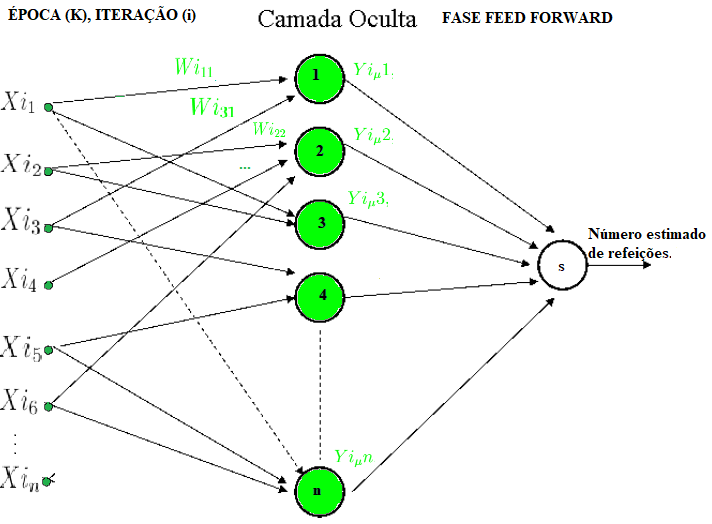
\includegraphics[width=0.65\textwidth]
          		{18-mlp-bp-ff1.png}
          	}
          	\caption{Apresentação da i-ésima observação do conjunto de treino à rede}
           \end{figure}
           
           \begin{figure}[!ht]
          	\center{
          		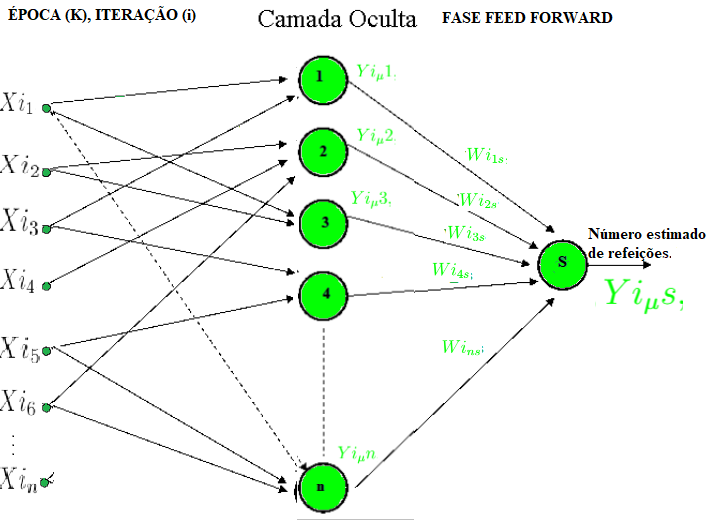
\includegraphics[width=0.65\textwidth]
          		{18-mlp-bp-ff2.png}
          	}
          	\caption{Cálculo do valor estimado de saída da rede.}
           \end{figure}
            
            O valor de $Yi_{\mu}(j)$. dos neurônios da primeira camada oculta, são obtidos de forma que $Xi_{n}(j)$ são os sinais de entrada das variáveis de 1 à $n$.
            
            O valor de $Yi_{\mu}(j)$. dos neurônios das próximas camadas, inclusive a de saída, utiliza o sinal de saída $Yi_{\mu}$ dos neurônios da camada anterior conectados à $j$ como um sinal de entrada $Xi_{n}$.
            
            %%%%%%%%%%%%%%%%%%%%%%%%%%%%%%
            \paragraph*{Fase Feedbackward}
            O Processo de reajuste dos pesos sinápticos com o objetivo de atingir a minimalização do erro quadrático da validação, é feito pelo método do Gradiente Descendente, reajustando os pesos sinápticos $Wi_{n}(j)$ correspondente à cada neurônio $j$ da rede, para um valor $\Delta Wi_{n}(j)$, da seguinte forma:\\
            $\Delta Wi_{n}(j) = \eta*\delta_j*Xi_{n}(j)$\\
            
            \subparagraph*{Regra $\delta$ para neurônio de saída}
            Exclusivamente para a camada de saída, $\delta$ é calculado por\\
            $\delta_s = (Yi - Yi_{\mu}(s) )*F'(\mu(s))$.
            \begin{figure}[!ht]
          	\center{
          		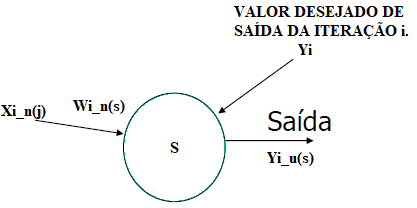
\includegraphics[width=0.40\textwidth]
          		{17-mlp-bp-saida.png}
          	}
          	\caption{Aprendizado de um neurônio na camada de saída}
           \end{figure}
            
            O valor dos $n$ pesos $Wi_{n}(s)$ do neurônio de saída $s$ com $n$ entradas vindas das saídas de neurônios $j$ das camadas anteriores, é obtido por $\Delta Wi_{n}(s) = \eta*\delta_s*Yi_{\mu}(j)$\\.
            \begin{figure}[!ht]
          	\center{
          		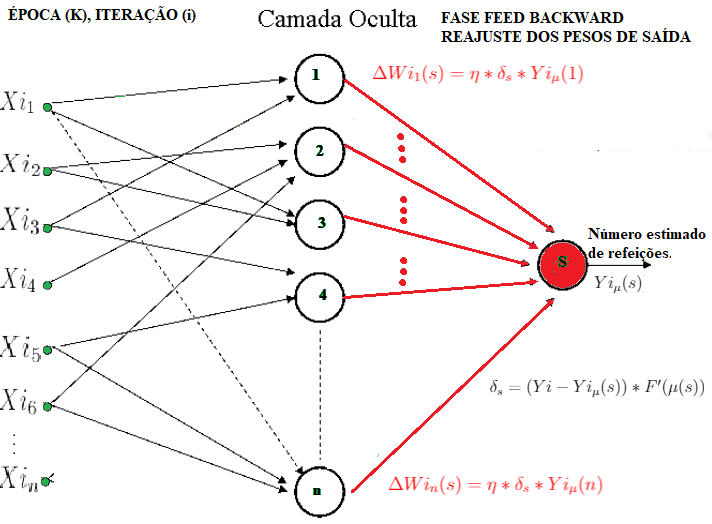
\includegraphics[width=0.65\textwidth]
          		{20-mlp-bp-fb.png}
          	}
          	\caption{Reajuste dos pesos de saída}
           \end{figure}
           %%%%%%%%%%%%%%%%%%%%%%%%%%%%%%%%%%%%%%%%%%%%%%%%%%%%%%%%%%%%%%%%
           \subparagraph*{Regra $\delta$ para neurônios de camadas ocultas}
            Nesta etapa, os neurônios $n$ da camada oculta obterão seu $\delta$ através da seguinte equação usando o $\delta$ dos $m$ neurônios da camada posterior que se conectam à ele:\\ 
            
            $\delta_n = F'(\mu(n))*(\sum \delta_m*Wi_{n}m)$\\
            
            Na rede neural de 1 camada oculta e 1 neurônio de saída, a soma será reduzida à apenas 1 neurônio, ficando então a regra $\delta$ da seguinte forma:\\
            
            $\delta_n = F'(\mu(n))*(\delta_s*Wi_{n}s)$\\
            
            Por fim os pesos das $n$ entradas $Wi_{n}(n)$ conectadas ao neurônio $n$ terão seus pesos reajustados da seguinte forma:\\
            $\Delta Wi_{n}(n) = \eta*\delta_n*Xi_{n}(n)$\\
            
            Após o reajuste chegar na primeira camada oculta, um novo vetor de observações $i$ é apresentado à rede repetindo, iniciando novamente a fase feed-forward e repetindo o ciclo até o fim das entradas.
            
            \begin{figure}[!ht]
          	\center{
          		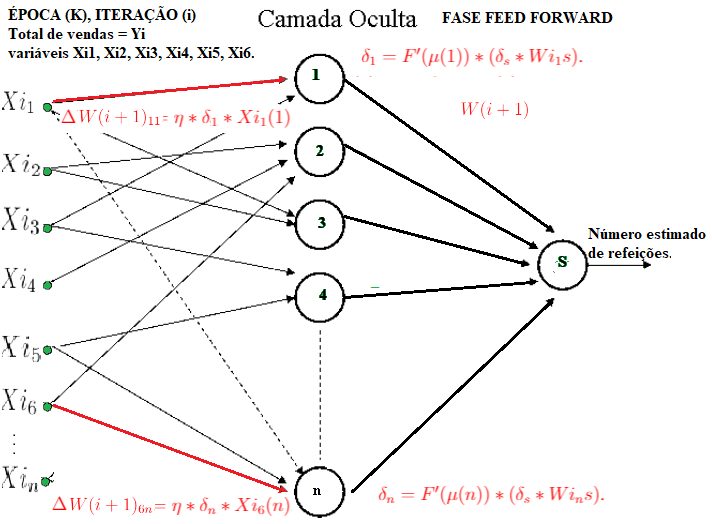
\includegraphics[width=0.65\textwidth]
          		{21-mlp-bp-fbe.png}
          	}
          	\caption{Reajuste dos pesos de camadas ocultas}
            \end{figure}
           
            \subparagraph{Validação de treino}
            Após se encerrar uma época, que percorreu todas as i-ésimas entradas do conjunto de treino, um conjunto de dados de validação, previamente separado, é apresentado à rede.
            A validação ocorre só com a fase feedforward, obtendo-se os erros quadráticos da camada de saída com o dado de validação observado.
            Então é calculado o $m.s.e$, obtendo-se a média de todos os i-ésimos erros quadráticos do conjunto de validação.
            O valor $m.s.e$ deve ser acompanhado até que se atinja um ponto ótimo, ou seja, um limite inferior após k épocas.
            Quando este limite for atingido em uma época $k_o$, todos os parâmetros da rede dentro da época $k_o$ serão os parâmetros desejados do modelo final da rede.
            
            Quando a curva do $m.s.e$ estiver sendo realizada, não se saberá o ponto ótimo de parada, até que ele comece a ser superado, logo é importante arbitrar um número $l$ para salvar os parâmetros das $l$ épocas anteriores.
        
        \subsection{Algoritmo de treino e validação backpropagation}
            Parâmetros de entrada:
            \begin{itemize}
                \item 'rna'[][], Grafo de nós do tipo neurônio, da rede neural, onde rna[m][n] corresponde ao nó "n" da camada "m".
                \item $\eta$, Taxa de aprendizado .
                \item Yt[][] e Yv[][], Matrizes Yt do conjunto de treino e Yv do conjunto de validação, onde Y[0][0] corresponde ao primeiro valor supervisionado, e Y[0][m] corresponde ao último parâmetro X relacionado ao valor supervisionado.
                \item L, Limite de armazenamento de épocas, para uma lista de tamanho L, de grafos 'rna' contendo a cópia de todos os parâmetros da rede.                
            \end{itemize}

            Será criado uma fila circular que irá armazenar cópias dos parâmetros da rede, da época vigente. Retornando os parâmetros da cópia corresponte ao ponto ótimo de parada.

            Nos passos abaixo, o critério de parada do treino (laço raiz) irá interromper o treino com o auxílio de uma fila circular de valores $m.s.e$.
            Essa fila circular mse de tamanho L é criada, percorrendo a curva m.s.e em função do aumento de épocas de treino, armazenando valores do $m.s.e$. Se L for suficientemente grande para compensar as oscilações de validação, quando a segunda metade dessa fila estiver totalmente após o ponto ótimo de parada, a soma dos valores desta segunda metade será maior que a soma dos valores da primeira metade. E assim o laço irá parar.

            Como a fila de cópias da rede avança simultaneamente com a fila de mse, a cópia contida na posição $\frac{L}{2}$ será a rede com os parâmetros ótimos, do ponto ótimo de treino.

            \begin{enumerate}
                \item Inicialize uma fila circular de grafos 'rna' de tamanho L, K[L].
                \item Inicialize uma fila circular com zeros, do tipo real, $m.s.e$ de tamanho L, mse[L].
                \item Copie 'rna'[][] para K[0].
                \item Inicialize uma variável inteira, contador de épocas, ck = 0.
                \item Inicialize uma variável inteira, errok.
                \item Insira uma cópia de 'rna'[][] para K[]
                
                \item LAÇO: Enquanto soma (mse[0] à mse[$\frac{L}{2}$]) for maior que (mse[$\frac{L}{2} +1$] à mse[L]) faça:
                \item   LAÇO: Percorra it[] em Yt[i].
                \item     Se i=0, inicialize os pesos de K[atual] com valores aleatoriamente pequenos. 
                \item     Execute a fase feedforward apresentando it[] em K[atual] e guarde o erro em errok.
                \item     Execute a fase feedbackward reajustando os pesos de K[atual] com errok.

                \item   Inicialize um vetor temporario ev[] de tamanho Yv[].tamanho, a quantidade de observações de treino.

                \item   LAÇO: Percorra iv[] em Yv[i].
                \item     Execute a fase feedforward apresentando iv[] em K[atual] e insira o erro quadrático em ev[i].

                \item   Obtenha a média dos valores quadráticos do vetor ev[] e insira em mse[]
                \item   Destrua ev[].
                \item   Insira uma cópia de K[atual] atual em K[].
                \item   incremente ck, ck=ck+1.

                \item Retorne K[$\frac{L}{2}$]
            \end{enumerate}

  % ----------------------------------------------------------
  % Trabalhos relacionados
  % ----------------------------------------------------------
  \chapter{Trabalhos relacionados}
    \subsection{ANÁLISES EM RESTAURANTES UNIVERSITÁRIOS}
        \paragraph*{} No estudo estatístico feito por \cite{Landim2016}, foi analisada a correlação entre a temperatura e o consumo nos dias de vendas do restaurante universitário do campus ICT da Unifesp, sendo que os dados continham uma amostra das vendas do segundo semestre de 2016. Devido ao baixo volume de ocorrências, os dados foram submetidos à reamostragem via bootstrap. De acordo com os gráficos das amostras, identificou-se que a correlação mostrada nos gráficos da primeira metade do semestre e do período total do semestre formaram distribuições bimodais. Porém, na segunda metade do semestre formou-se uma distribuição unimodal. Portanto, concluiu-se que outras variáveis e outros modelos de análises podem ser utilizados para tal análise de demanda.
        
        \paragraph*{} \cite{Lopes2008} faz o mesmo estudo deste cenário do ICT UNIFESP aplicado na Universidade Federal de Viçosa (UFV). Neste estudo, os dados utilizados foram somente o histórico de vendas do restaurante universitário, e nenhuma variável de ambiente foi coletada como temperatura, precipitação, número de alunos matriculados, etc. O algoritmo utilizado foi o Traincgp (Conjugate gradient backpropagation with Polak-Ribiere updates) no software Matlab. Este algoritmo não envolve o cálculo das derivadas segundas das variáveis e converge ao mínimo da função quadrática em um número finito de iterações como cita o autor. Foram então considerados para cada nó da rede neural, o dia da semana (como segunda, terça, quarta, quinta e sexta) e cada camada dessa rede utilizando os 5 dias anteriores para cada nó (as 5 segundas anteriores, 5 terças anteriores e assim sucessivamente) e, por fim, obtido um modelo pela rede que apresentou erro máximo de 3.
        
        \paragraph*{} \cite{Rocha2011} também realiza o estudo de demanda no restaurante universitário da Universidade Estadual Paulista Júlio de Mesquita Filho (UNESP), novamente com os métodos de redes neurais artificiais com backpropagation, e utilizando apenas como fonte de dados o histórico numérico das vendas realizadas, e outras variáveis intermediárias obtidas a partir deste como médias de subconjunto de observações (médias de segundas-feiras), e a única variável de ambiente coletada foi o número de feriados próximos à observação de venda. No estudo do total de dias analisados, verifica-se que em 73\% (187 dias), o método de média simples propiciou um maior erro em relação à RNA, que por sua vez ocasionou um erro maior nos 23\% (69 dias) restantes.Em se tratando de menor desperdício, observa-se que a RNA apresenta erros maiores que 50 refeições em 13 dias, enquanto o método da média simples apresenta erros maiores que 50 refeições em 58 dias, concluindo-se então que o método de RNA foi bem mais eficiente do que o cálculo de média simples utilizado pela administração do restaurante universitário.
      
      \subsection{ANÁLISES EM OUTROS CENÁRIOS} 
        \paragraph*{} \cite{Ruas2012} fazem uma análise de previsão de demanda de energia elétrica no estado do paraná, entre os anos de 2004 e 2006, utilizando redes neurais artificiais e máquinas de vetores de suporte. Apesar de não ser o mesmo exemplo do cenário do restaurante universitário do ICT UNIFESP, temos na distribuição dos dados de consumo coletados como uma série temporal, e foi utilizado nesta pesquisa uma rede parcialmente recorrente de Elman, que permite a previsão de um passo de tempo à frente. Para que seja possível realizar a previsão vários pontos à frente, é necessário utilizar os valores já previstos, ou seja, a saída da rede, como entradas da mesma. Logo, como o cenário da demanda do RU no ICT UNIFESP se apresenta como uma série temporal e tentaremos prever a demanda um passo à frente, será interessante a este trabalho utilizar e comparar as técnicas previstas nesta referência.
        
        \paragraph*{} \cite{Almeida2013} analisa um cenário semelhante de demanda de energia elétrica, porém utilizando-se técnicas de previsão de demanda com Rede Neural Artificial do tipo Multilayer Perceptron combinado com lógica fuzzy que permite colocar variáveis de temperatura (entre outras) em um conjunto de regras que impactam no problema. Esta análise é interessante pois é semelhante à referência 2 que faz um estudo com redes neurais perceptron no mesmo tema deste trabalho de conclusão de concurso, mas com a adição da lógica fuzzy que permite utilizar outras variáveis de ambiente impactantes, que não sejam somente o histórico numérico do consumo.
        
        \paragraph*{} \cite{Silva2010} também aplica técnicas de redes neurais para previsão de demanda de energia elétrica, com o estudo de variáveis climáticas, porém através de um modelo de MAPA SOM - (Self-Organizing Map) que é um tipo de rede neural desenvolvido para reconhecimento de padrões. Apesar de ser um modelo não supervisionado, o modelo é ideal para organizar as principais variáveis impactantes e descartáveis na previsão. O mapa som utilizado pelo autor apresenta os dados associados aos seus neurônios de forma que padrões similares encontram-se em neurônios contíguos, tendo uma organização topológica. Deste modo é possível se extrair relações abstratas entre as variáveis do vetor de dados através da sua posição nos mapas componentes, que por meio de uma escala de cores mostram a quantidade de uma variável específica em cada neurônio do mapa.
       
       \subsection{TESES COMPARATIVAS DE DIVERSOS MÉTODOS DE PREVISÃO DE DEMANDA.}
        \paragraph*{} \cite{Junior2007} realiza um trabalho de comparação entre diversas técnicas de Métodos estocásticos e Rede Neural Artificial (RNA), para a previsão da demanda de produtos cosméticos, distribuídos em séries temporais. Entre eles Redes Neurais tipo feedforward, com o algoritmo backpropagation que foi o principal foco no trabalho de previsão de RU na Universidade Federal de Viçosa e na Universidade Estadual Paulista Júlio de Mesquita Filho. Será realizado a análise dessas comparações e seleção de principais algoritmos que possam ser aplicados e comparados neste trabalho.
        
  % entre os dados previstos e observados.
  % ----------------------------------------------------------
  % \chapter{Plano de atividades para o TCC II}
  % ----------------------------------------------------------
  \chapter{Plano de atividades para o TCC II}
    Para a continuação deste trabalho o cronograma abaixo deve ser seguido.

    \begin{table}[!ht]
    	\centering
    		\caption{Plano de atividades para o TCC II}	\label{tab:plano}
    		\begin{tabular}{|c|c|c|c|c|c|c|}
    			\hline  \textbf{Atividades} &	\textbf{Março} &	\textbf{Abril} & \textbf{Maio} & \textbf{Junho} & \textbf{Julho} \\
    			\hline 1 & $\checkmark$ 	& & & & 	\\
    			\hline 2 & $\checkmark$	& & & & 	\\
    			\hline 3 & 	&$\checkmark$ &$\checkmark$ & & 	\\
    			\hline 4 & 	&$\checkmark$ &$\checkmark$ &$\checkmark$ & 	\\
    			\hline 5 & 	&$\checkmark$ &$\checkmark$ &$\checkmark$ & 	\\
                \hline 6 &  & & & &$\checkmark$ 	\\
    			\hline 
    		\end{tabular}
    \end{table}
    \begin{enumerate}
    
    \item Estruturação do conjunto de dados do R.U do ano de 2017 conforme fundamentado na seção de estruturação de dados linear múltipla. O carregamento dos dados será realizado no Matlab, que já tem bibliotecas prontas que retornam o dia da semana baseado em uma data de entrada. Realizar predição de regressão com dados de 2017 e validar com 2018. Anotando-se o Erro Absoluto Médio (EAM), Erro Quadrado Médio (EQM) e Raiz do Erro Quadrado Médio (REQM).
    
    \item O conjunto de dados estruturado na etapa anterior, terá um conjunto de 20\% de observações retiradas de cada estação do ano de 2017. Serão formados através do conjunto original, 3 pares de conjunto treino - validação.
    
    \item Implementação do grafo rede neural com nós perceptrons. Cada nó deve conter métodos de inicialização do número de entradas, inicialização dos pesos, inicialização de função de ativação, inicialização de bias e calculo de saída. O grafo deve conter métodos de criar camadas, nós em cada camada, criar arestas orientadas das conexões dos nós.

    \item Implementação do método feedforward que deve ser capaz de percorrer as camadas do grafo, e calcular o sinal de saída.

    \item Implementação do método feedbackward que deve ser capaz de percorrer inversamente as camadas do gravo, e regravar os pesos sinápticos de cada nó.

    \item Implementação do Algoritmo de treino e validação backpropagation

    \item Execução 

    \end{enumerate}

     estrutura de dados perceptron, será criado 3 perceptrons, cada perceptron será associado com cada par de conjunto-treino validação gerado aleatoriamente do conjunto original, e implementar a função de treino perceptron simples. A função treino irá reajustar os pesos de cada perceptron. Com os perceptrons com pesos reajustados, todos os 3 irão receber um vetor de entradas de variáveis preditivas de 2018, e emitirão uma saída k1, k2 e k3. Será feita uma média aritmética da saída k1, k2 e k3, obtendo-se km que será comparado com a saída desejada Yi de 2018. Anotando-se o Erro Absoluto Médio (EAM), Erro Quadrado Médio (EQM) e Raiz do Erro Quadrado Médio (REQM) de Yi com Km.

  % ----------------------------------------------------------
  % \chapter{Plano de atividades para o TCC II}
  % ----------------------------------------------------------
  \chapter{Conclusão}
    .

  %\begin{itemize}
  %\item Contextualização e Motivação; 
  %\item Definição do problema; 
  %\item Justificativas;
  %\item Objetivos:  Geral e específicos;
  %\item Metodologia e
  %\item Organização do documento.
  %\end{itemize}

  %\subsection{Sobre os Títulos e Capítulos}

  %As demais subdivisões do texto (seções, subseções, etc) ... 

  %\subsubsection{Título de Subseção}
  %Veja aqui um exemplo de citaçao direta \cite{memoir}.


  % ----------------------------------------------------------
  % Capitulo com exemplos de comandos inseridos de arquivo externo 
  % ----------------------------------------------------------

  % ---
  % Capitulo de revisão de literatura
  % ---
  %\chapter{Revisão Bibliográfica}

  % ---
  %\section{Introdução}
  % ---

  % ---
  % primeiro capitulo de Resultados
  % ---
  %\chapter{Resultados}

  % ---
  % Finaliza a parte no bookmark do PDF, para que se inicie o bookmark na raiz
  % ---
  \bookmarksetup{startatroot}% 
  % ---

  % ---
  % Conclusão
  % ---

  % ----------------------------------------------------------
  % ELEMENTOS PÓS-TEXTUAIS
  % ----------------------------------------------------------
  %\postextual


  % ----------------------------------------------------------
  % Referências bibliográficas
  % ----------------------------------------------------------
  %\bibliographystyle{plain}
  \bibliography{references}

  % ----------------------------------------------------------
  % Glossário
  % ----------------------------------------------------------
  %
  % Consulte o manual da classe abntex2 para orientações sobre o glossário.
  %
  %\glossary

  % ----------------------------------------------------------
  % Apêndices
  % ----------------------------------------------------------

  % ---
  % Inicia os apêndices
  % ---
  %\begin{apendicesenv}

  % Imprime uma página indicando o início dos apêndices
  %\partapendices

  % ----------------------------------------------------------
  %\chapter{Título de Apêndice}
  % ----------------------------------------------------------


  % ----------------------------------------------------------
  %\chapter{Título do Apêndice}
  % ----------------------------------------------------------


  %\end{apendicesenv}
  % ---


  % ----------------------------------------------------------
  % Anexos
  % ----------------------------------------------------------

  % ---
  % Inicia os anexos
  % ---
  %\begin{anexosenv}

  % Imprime uma página indicando o início dos anexos
  %\partanexos

  % ---
  %\chapter{Título do Anexo}
  % ---

  %\end{anexosenv}

  \end{document}